% !TEX root = ../sablona-prace.tex

\chapter{Implementace řídícího algoritmu}
Podle popsaných principů jsem vytvořil Simulink kód a knihovnu jednotlivých bloků, schéma implementovaného řízení je na obrázku \ref{fig:impl_blokove_schema}.

\input{obrazky/impl_blokove_schema}

Pro práci jsem použil Matlab Simulink R2025b. Parametry simulace jsou inicializovány ve skriptu \texttt{ParamInit}. Ten využívá některých konstant předpočítaných v jiných skriptech jako  data MTPA tabulky, tabulka pro určení sektoru svm, pole vektorů pro jednotlivé sektory a podobně.

Nejdříve jsem vytvořil spojité varianty základních funkcí SVM, převodní matice, regulátor proudu. Ty jsem otestoval na simscape modelu od Mathworks.
Poté jsem tyto bloky převedl do verze vhodné pro generování HDL kódu, bloky využívají datových typů s pevnou desetinnou čárkou, a pouze funkce podporované pro generování HDL kódu.

Protože simscape model Matlabu nesimuluje vliv 3. harmonické byl jsem nucen pro další postup přejít na vlastní model, ten jsem vytvořil využitím  popisu motoru  v dq13.

Všechny moduly řízení vrací výstup za jednu modulační periodu označenou v inicializačním skriptu jako $T_s$. Pro tuto práci byl tento čas nastaven na $50\,\mu\text{s}$.

Následně jsem dodělal už pouze diskrétní bloky pro generování vektoru referenčních napětí a otestoval funkčnost kompletního řízení otáček simulovaného motoru.

Pro otestované bloky jsem jednotlivě vygeneroval IP bloky, a ty nahrál na ZedBoard a jednotlivě ověřil jejich funkčnost. Na závěr jsem vytvořil jeden IP blok pokrývající celé  řízení. Ověřil že se celé řízení vydá na desku a otestoval jeho funkčnost.

Součástí elektronické přílohy je simulink knihovna s vytvořenými funkcemi, simulinkové schéma simulující celý systém poskládaný z HDL kompatibilních funkcí a pomocné soubory ze kterých byly vygenerovány konstanty pro jednotlivé bloky.


V kapitole níže jsou rozebrány detaily jednotlivých bloků, popsáno jejich chování a výpočetní náročnost. V tabulce u každého z bloků jsou pak shrnuty HW nároky jednotlivých bloků.



\section{Implementace transformačních matic}

\subsubsection{Transformace do $dq_{1\,3}$}
Měřený proud je po změření potřeba transformovat do $dq_{1,3}$ pro další bloky vektorového řízení. Transformace, jak bylo popsáno v kapitole \ref{kap:transformace}, spočívá v násobení proudového vektoru maticí $K_r$ \ref{mat:Kr impl}.

\begin{equation}
\label{mat:Kr impl}
 K_r=\resizebox{0.8\textwidth}{!}{$
    \left( \begin{array}{ccccc}
    \cos \left(\theta \right) & \cos \left(\theta -\frac{2\,\pi }{5}\right) & -\cos \left(\theta +\frac{\pi }{5}\right) & -\cos \left(\theta -\frac{\pi }{5}\right) & \cos \left(\theta +\frac{2\,\pi }{5}\right)\\
    -\sin \left(\theta \right) & \cos \left(\theta +\frac{\pi }{10}\right) & \sin \left(\theta +\frac{\pi }{5}\right) & -\cos \left(\theta +\frac{3\,\pi }{10}\right) & -\sin \left(\theta +\frac{2\,\pi }{5}\right)\\
    \cos \left(3\,\theta \right) & -\cos \left(3\,\theta -\frac{\pi }{5}\right) & \cos \left(3\,\theta -\frac{2\,\pi }{5}\right) & \cos \left(3\,\theta +\frac{2\,\pi }{5}\right) & -\cos \left(3\,\theta +\frac{\pi }{5}\right)\\
    -\sin \left(3\,\theta \right) & -\cos \left(3\,\theta +\frac{3\,\pi }{10}\right) & \cos \left(3\,\theta +\frac{\pi }{10}\right) & -\sin \left(3\,\theta +\frac{2\,\pi }{5}\right) & \sin \left(3\,\theta +\frac{\pi }{5}\right)
\end{array} \right)
$}
\end{equation} 

Jednotlivé prvky této matice jsou závislé na úhlu $\theta$, musí být proto spočítána pro každý časový okamžik znovu. To by znamenalo 20 přístupu do lookup tabulek. Aby byl omezen počet výpočtů $\sin$ a $\cos$, upravil jsem  matici $K_r$  do tvaru~\ref{mat:Kr hdl}, kde $k_1$ až $k_{5}$ jsou konstanty a ve výrazu se vyskytují pouze hodnoty $\sin(\theta)$, $\cos(\theta)$, $\sin(3\theta)$ a $\cos(3\theta)$. Tato úprava snižuje počet nutných výpočtů $\sin$ a $\cos$ z 20 na 4, neboť každý prvek původní matice obsahuje jiný úhel, zatímco upravený tvar závisí výhradně na těchto čtyřech hodnotách. Tyto hodnoty jsou získány z lookup tabulky předřazené před násobením. Výsledné simulinkové schéma je na obrázku~\ref{fig: ad2dq simulink}.


\begin{equation}
\label{mat:Kr hdl}
\resizebox{0.9\textwidth}{!}{$
K_r = \begin{pmatrix}
\cos(\theta) & k_1 \cos(\theta) + k_2 \sin(\theta) & k_3 \cos(\theta) + k_4 \sin(\theta) & k_3 \cos(\theta) - k_4 \sin(\theta) & k_1 \cos(\theta) - k_2 \sin(\theta) \\
-\sin(\theta) & k_2 \cos(\theta) - k_1 \sin(\theta) & k_4 \cos(\theta) + k_5 \sin(\theta) & -k_4 \cos(\theta) + k_5 \sin(\theta) & -k_2 \cos(\theta) - k_1 \sin(\theta) \\
\cos(3\theta) & k_3 \cos(3\theta) - k_4 \sin(3\theta) & k_1 \cos(3\theta) + k_2 \sin(3\theta) & k_1 \cos(3\theta) - k_2 \sin(3\theta) & k_3 \cos(3\theta) + k_4 \sin(3\theta) \\
-\sin(3\theta) & -k_4 \cos(3\theta) + k_5 \sin(3\theta) & k_2 \cos(3\theta) - k_1 \sin(3\theta) & -k_2 \cos(3\theta) - k_1 \sin(3\theta) & k_4 \cos(3\theta) + k_5 \sin(3\theta)
\end{pmatrix}
$}
\end{equation}
\noindent kde jednotlivé koeficienty jsou definovány jako: \\
\noindent    $k_1 = \frac{\sqrt{5}-1}{4}$,
     $k_2 = \frac{\sqrt{2}\sqrt{5+\sqrt{5}}}{4} $,
     $k_3 = -\frac{\sqrt{5}+1}{4} $,
    $ k_4 = \frac{\sqrt{2}\sqrt{5-\sqrt{5}}}{4}$


\begin{figure}[!h]
    \centering
    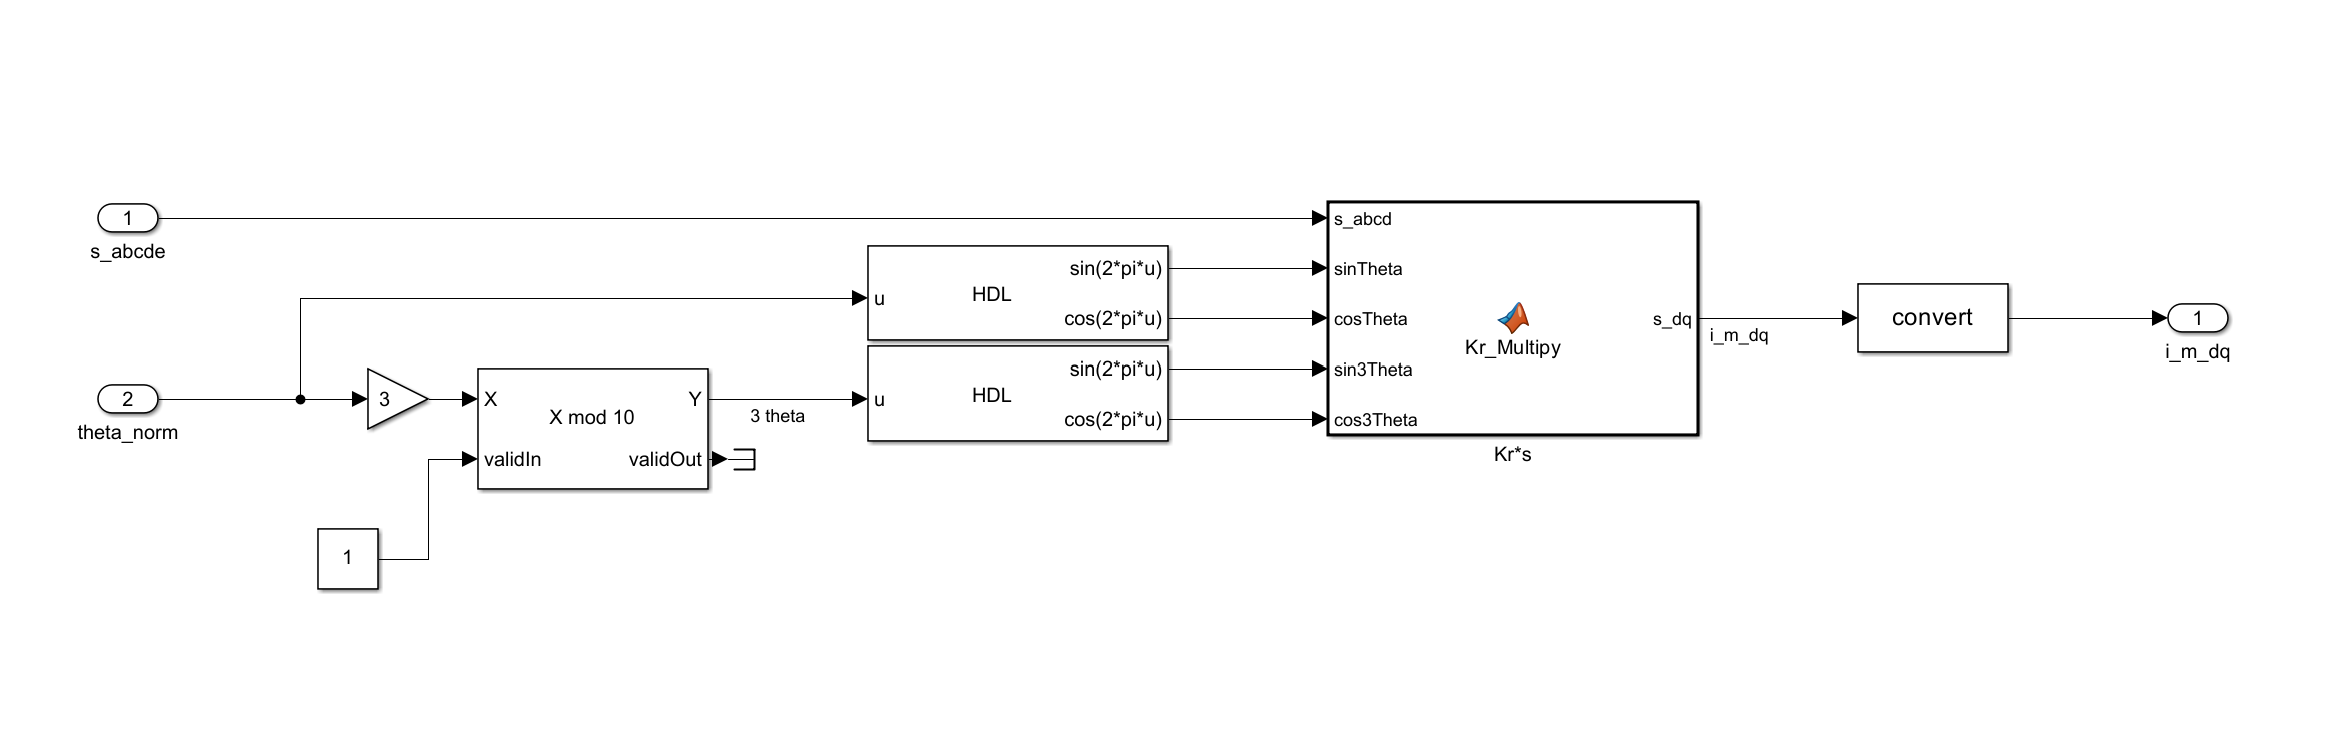
\includegraphics[width=\linewidth]{obrazky/abc2dq.png}
    \caption{Implementace převodu do $dq_{1\,3}$ uzpůsobeného pro HDL v Simulinku}
    \label{fig: ad2dq simulink}
\end{figure}

\begin{table}[htbp]
\centering

\begin{tabular}{lrrrr}
\toprule
\textbf{Prostředek} & \textbf{Použito} & \textbf{Dostupné} & \textbf{[\%]} \\
\midrule
Slice LUT (celkem)       & 8\,917 & 53\,200  & 16{,}76 \\
\quad z toho: logika     & 8\,730 & 53\,200  & 16{,}41 \\
\quad z toho: dist. RAM  &   126  & 17\,400  & 0{,}72 \\
\quad z toho: shift reg. &    61  & 17\,400  & 0{,}35 \\
Slice Registers (FF)     & 2\,918 & 106\,400 & 2{,}74 \\
Block RAM tile           &     0  &    140   & 0{,}00 \\
DSP48E1 (násobičky)      &    48  &    220   & 21{,}82 \\
Slice                    & 3\,342 & 13\,300  & 25{,}13 \\
\bottomrule
\end{tabular}
\caption{Využití HW prostředků FPGA -- na převod za $abcde$ do $dq_{1\,3}$ (\texttt{abc2dq})}
\label{tab:hw_hdl_projKR}
\end{table}

\subsubsection{Ostatní převodní matice}

Obdobným způsobem jsem vytvořil funkci \texttt{dq2AlphaBeta} pro převod napěťové reference z $dq_{1\,3}$ do $\alpha \beta_{1\,3}$ pro modulátor a funkci \texttt{dq2abcde} pro převod z $dq_{1\,3}$ do $abcde$.
Stejně jako $K_r$ jsem i matici $K_r^{inv}$ upravil do tvaru~\ref{mat:Kr inv hdl}, ve kterém lze všechny prvky vyjádřit jako součin konstant a hodnot $\sin(\theta)$, $\cos(\theta)$, $\sin(3\theta)$ a $\cos(3\theta)$. Matice $R_{inv}$ již vhodný tvar má, stačí pouze předpočítat hodnoty goniometrických funkcí a předat je MATLAB funkci jako parametr.

\begin{equation}
    \label{mat:Kr inv hdl}
    \resizebox{0.9\textwidth}{!}{$
    K_r^{inv} = \begin{pmatrix}
\cos(\theta) & -\sin(\theta) & \cos(3\theta) & -\sin(3\theta) \\
k_1 \cos(\theta) + k_2 \sin(\theta) & k_2 \cos(\theta) + k_3 \sin(\theta) & k_4 \cos(3\theta) + k_7 \sin(3\theta) & k_7 \cos(3\theta) + k_6 \sin(3\theta) \\
k_4 \cos(\theta) + k_5 \sin(\theta) & k_5 \cos(\theta) + k_6 \sin(\theta) & k_1 \cos(3\theta) + k_2 \sin(3\theta) & k_2 \cos(3\theta) + k_3 \sin(3\theta) \\
k_4 \cos(\theta) + k_7 \sin(\theta) & k_7 \cos(\theta) + k_6 \sin(\theta) & k_1 \cos(3\theta) + k_8 \sin(\theta) & k_8 \cos(3\theta) + k_3 \sin(3\theta) \\
k_1 \cos(\theta) + k_8 \sin(\theta) & k_8 \cos(\theta) + k_3 \sin(\theta) & k_4 \cos(3\theta) + k_5 \sin(3\theta) & k_5 \cos(3\theta) + k_6 \sin(3\theta)
\end{pmatrix}$}
\end{equation}
\noindent kde jednotlivé koeficienty jsou definovány jako: \\ 
\noindent $
k_1 = \frac{\sqrt{5}}{4} - \frac{1}{4} $, 
$k_2 = \frac{\sqrt{2} \sqrt{\sqrt{5}+5}}{4} $,
$k_3 = \frac{1}{4} - \frac{\sqrt{5}}{4} $,
$k_4 = -\frac{\sqrt{5}}{4} - \frac{1}{4} $,
$k_5 = \frac{\sqrt{2} \sqrt{5-\sqrt{5}}}{4} $,
$k_6 = \frac{\sqrt{5}}{4} + \frac{1}{4} $,
$k_7 = -\frac{\sqrt{2} \sqrt{5-\sqrt{5}}}{4} $,
$k_8 = -\frac{\sqrt{2} \sqrt{\sqrt{5}+5}}{4}$,

\begin{table}[h]
\centering

\begin{tabular}{lrrrr}
\toprule
\textbf{Prostředek} & \textbf{Použito} & \textbf{Dostupné} & \textbf{[\%]} \\
\midrule
Slice LUT (celkem)       & 2\,106 & 53\,200  & 3{,}96 \\
\quad z toho: logika     & 1\,921 & 53\,200  & 3{,}61 \\
\quad z toho: dist. RAM  &   124  & 17\,400  & 0{,}71 \\
\quad z toho: shift reg. &    61  & 17\,400  & 0{,}35 \\
Slice Registers (FF)     & 2\,668 & 106\,400 & 2{,}51 \\
Block RAM tile           &     0  &    140   & 0{,}00 \\
DSP48E1 (násobičky)      &    48  &    220   & 21{,}82 \\
Slice                    & 1\,083 & 13\,300  & 8{,}14 \\
\bottomrule
\end{tabular}
\caption{Využití HW prostředků FPGA pro převod z $dq_{1\,3}$ do$\alpha \beta _{1\,3}$  (\texttt{dq2alphabeta})}
\label{tab:hw_hdlKrinv}
\end{table}

\subsubsection{Ověření transformace}
Pro ověření transformace jsem v simulaci roztočil motor kladným směrem působením vnějšího momentu. Vstupy motoru jsem nechal nepřipojené a měřil jsem indukované napětí, to jsem transformoval do $dq$. Tím jsem si ověřil správný převod a ověřil případný offset magnetického pole statoru vůči snímači otáček. Při tom jsem zjistil, že simscape model, který jsem chtěl původně použít, negeneruje napětí ve 3.\,harmonické.


\section{SVM modulátor}
Jak je popsáno v kapitole~\ref{kap:svm}, pro výpočet časů sepnutí jednotlivých fází je nutné zjistit sektor, ve kterém se požadované napětí nachází, spočítat časy aplikace jednotlivých vektorů a následně na základě zvolených vektorů a jejich časů určit časy sepnutí jednotlivých tranzistorů. Implementace modulátoru v Simulinku je na obrázku~\ref{fig:simulink svm}.

\begin{figure}[h]
    \centering
    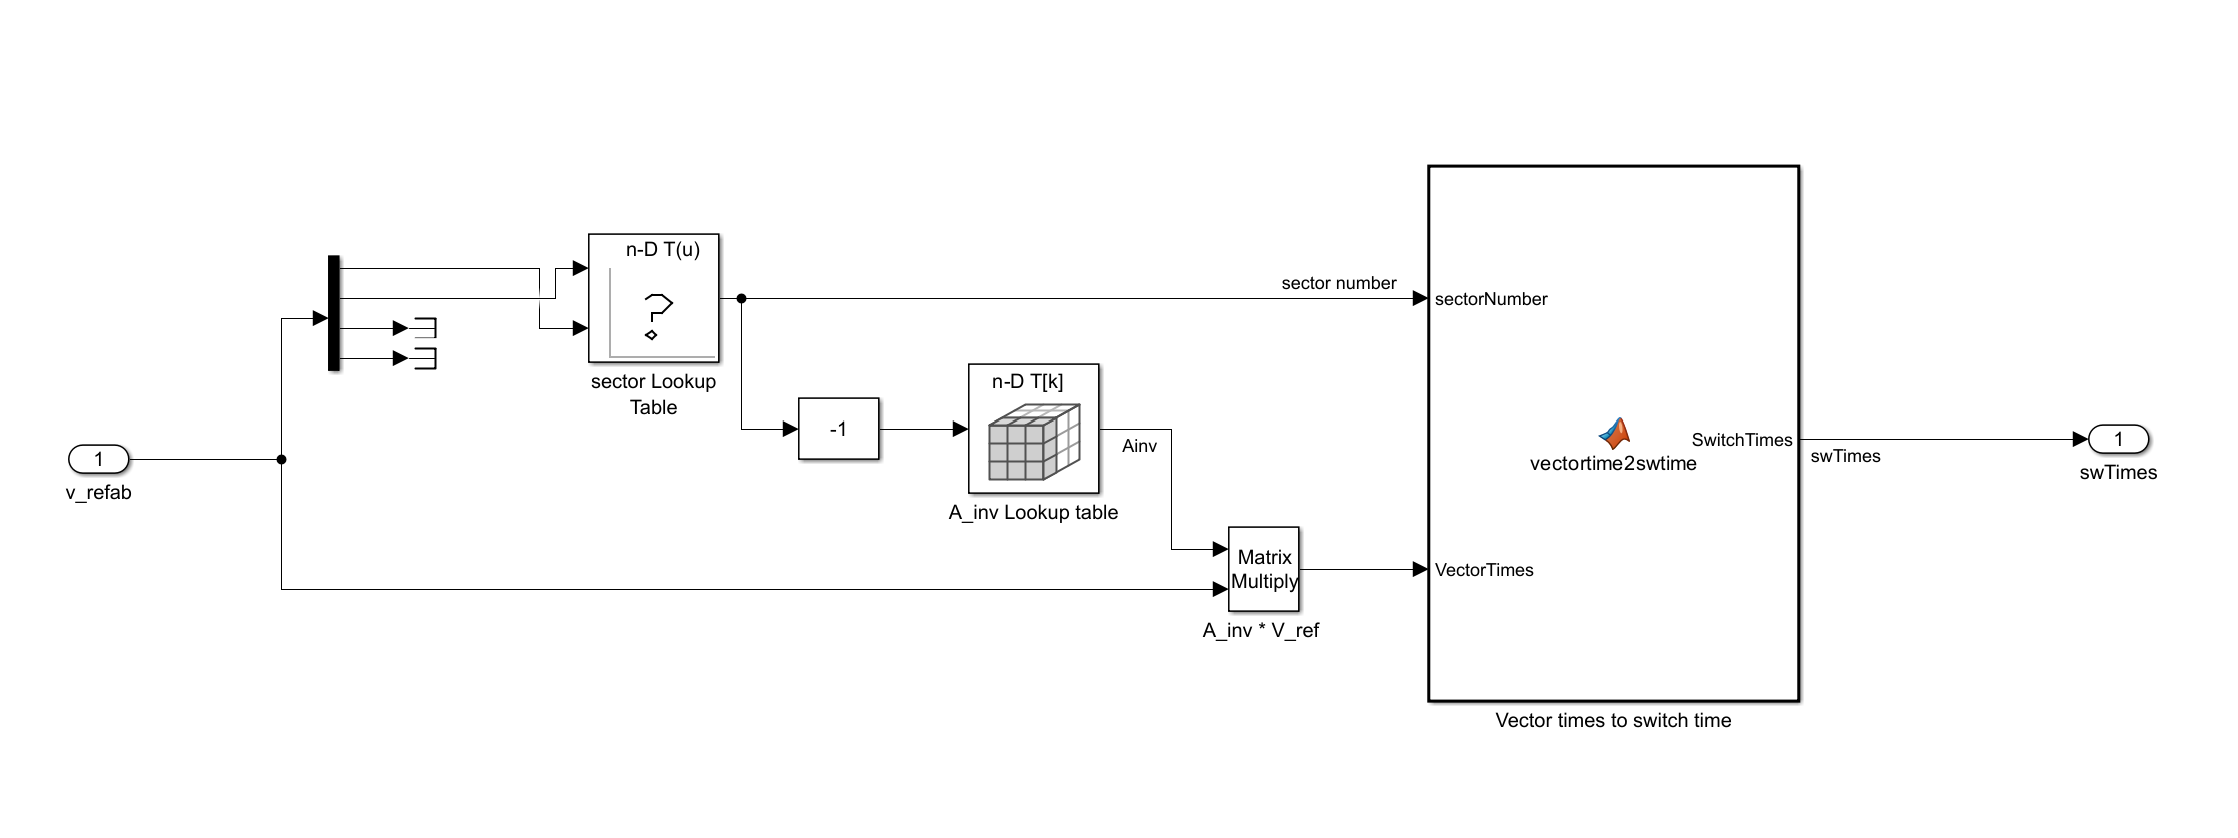
\includegraphics[width=\linewidth]{obrazky/svm_simulink.png}
    \caption{Implementace SVM v Simulinku po úpravě pro HDL}
    \label{fig:simulink svm}
\end{figure}
 

Sektor lze určit z úhlu vektoru vůči ose $\alpha_1$, to však obnáší výpočet úhlu $\gamma = \mathrm{arctg}\left(\frac{v_\beta}{v_\alpha}\right)$. Dělení i $\mathrm{arctg}$ jsou v HDL zbytečně složité operace, proto jsem vytvořil 2D lookup tabulku, která ke každé možné kombinaci $v_{\alpha}$ a $v_{\beta}$ přiřadí odpovídající sektor.

Pro výpočet časů vektorů je zapotřebí inverze matice $A_n$ (vztah~\ref{eq: prirazeni svm}). Aby se předešlo výpočtu $\sin$, $\cos$ a inverze za běhu, byly matice $A_{n-inv}$ předpočítány pro každý z 10 sektorů. Z lookup tabulky je poté vybrána matice odpovídající danému sektoru.

Vynásobením požadovaného vektoru s maticí $A_{n-inv}$ pak získám požadovaný čas aktivace daného vektoru. V Matlab funkci \texttt{vectortime2swtime} jsou poté na základě čísla sektoru z předpočítaných polí vybrány aktivní vektory a jim odpovídající kombinace spínačů. Na základě znalostí těchto aktivačních vektorů a jim příslušných časů, jsou pak ve funkci dopočítány časy sepnutí jednotlivých fází, podle rovnice \ref{eq:swtime}. 

Zbylý čas, po který není aktivní ani jeden z vybraných vektorů, je rozdělen mezi 2 nulové vektory $U_0$ a $U_{31}$.

\begin{equation}
    t_{sw}= [u_1 u_2 u_3 u_4]  \cdot t_{vec}+ \frac{t_0}{2}
    \label{eq:swtime}
\end{equation}

Kde $t_{sw}$ je sloupcový vektor odpovídající výsledným časům sepnutí jednotlivých fází, $u_n$ jsou sloupcové vektory odpovídající jednotlivým výstupním vektorům, $t_{vec}$ je již vypočítaný čas aktivace jednotlivých vektorů a $t_0$ je čas připadající na nulové vektory.

Zároveň je v bloku \texttt{vectortime2swtime} ošetřen stav, kdy vyjde záporný čas aplikace některého z vektorů. Pokud je čas aplikace některého vektoru záporný, je daný vektor $u_i$  nahrazen vektorem opačným.

Výstupem bloku jsou vypočítané časy sepnutí jednotlivých fází nabývající hodnot z intervalu $\langle 0, 1 \rangle$, kde 1 odpovídá délce modulační periody. Ukázka výstupu pro $V_{dq}=[20;0;0;0]^T$ je na obrázku \ref{fig:out svm}. Takto normované časy jsou následně předány bloku HW interface, který z nich generuje řídicí signály jednotlivých tranzistorů.

\begin{figure}[h]
    \centering
    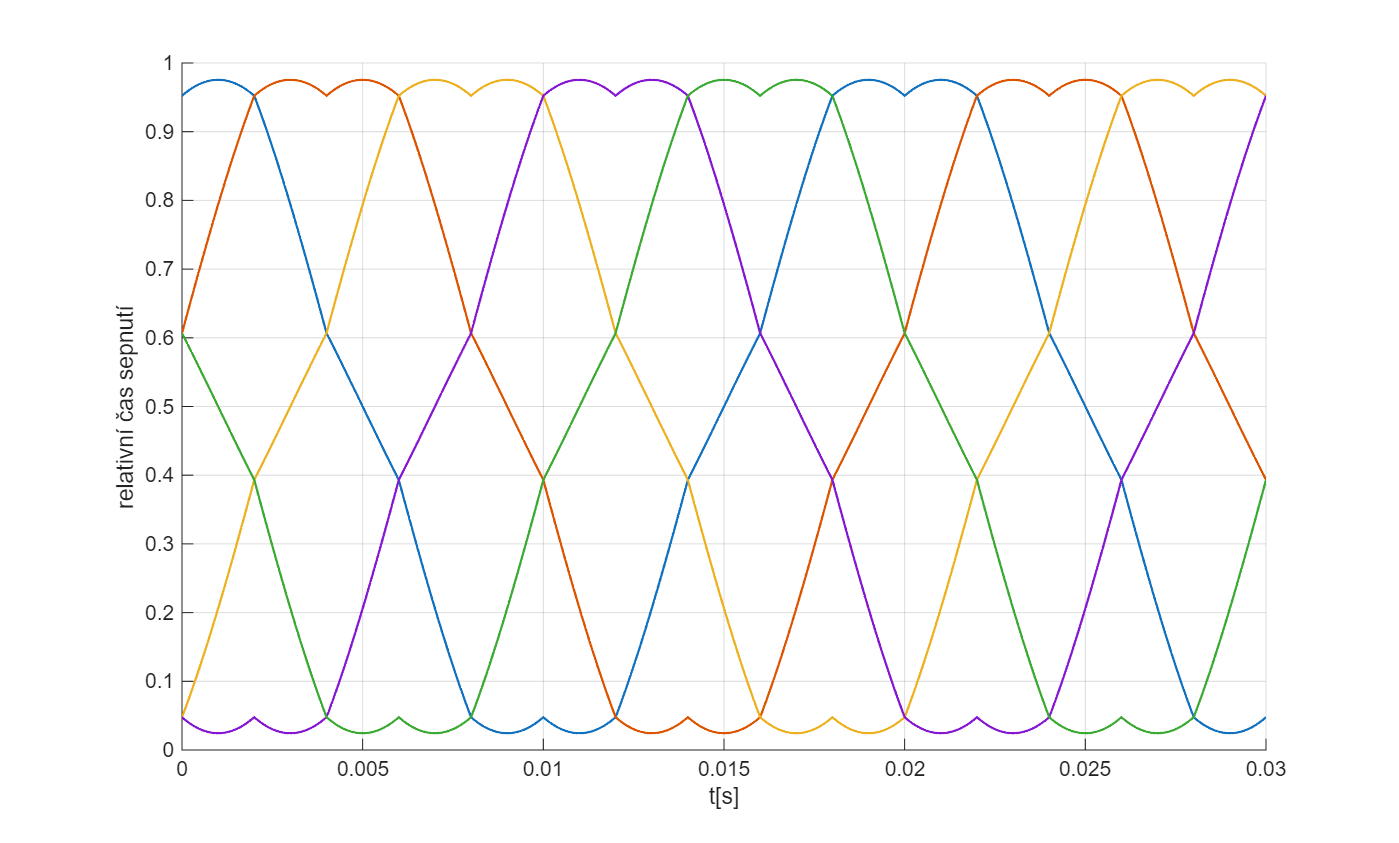
\includegraphics[width=  \linewidth]{obrazky/svm_t.png}
    \caption{Ukázka generovaných časů sepnutí jednotlivých fází pro $V_{dq}=[20;0;0;0]^T$}
    \label{fig:out svm}
\end{figure}

\section{Vyvedení výstupu modulátoru}
\label{kap:vyvedeni}
Vypočítané časy sepnutí jednotlivých fází je nutné dále převést na signály pro spínání tranzistorů, případně na akční zásah pro simulátor. To zajišťuje blok \texttt{HW\_interface\_xxxx}. Tento blok jsem vytvořil v několika verzích
v závislosti na využití: pro zjednodušenou simulaci, pro simulaci včetně střídače a verze s výstupem na fyzický pin ZedBoardu.

Všechny bloky vyvedení výstupu využívají stejného principu symetrické modulace. Symetrická modulace zajišťuje, že každý spínací impulz je symetricky umístěn kolem středu modulační periody, čímž se ve výstupním napětí potlačují sudé harmonické složky\cite{}. Požadovaný čas sepnutí je porovnáván se stavem čítače, který během modulační periody dokončí cyklus od 0 do 1 a zpět. Díky tomu je spektrum výstupního napětí čistší. Výstupem je signál, který označuji jako $sw_i$, kde $i$ odpovídá číslu fáze.
Pokud je $sw_i$ roven 1, na výstupu je $\frac{V_{dc}}{2}$, pokud je roven 0, na výstupu je $\frac{-V_{dc}}{2}$.
Příklad výstupu je zobrazen na obrázku \ref{fig: sym modulace}, pro přehlednost jsou na obrázku viditelné pouze první 2 fáze.

\begin{figure}[h]
    \centering
    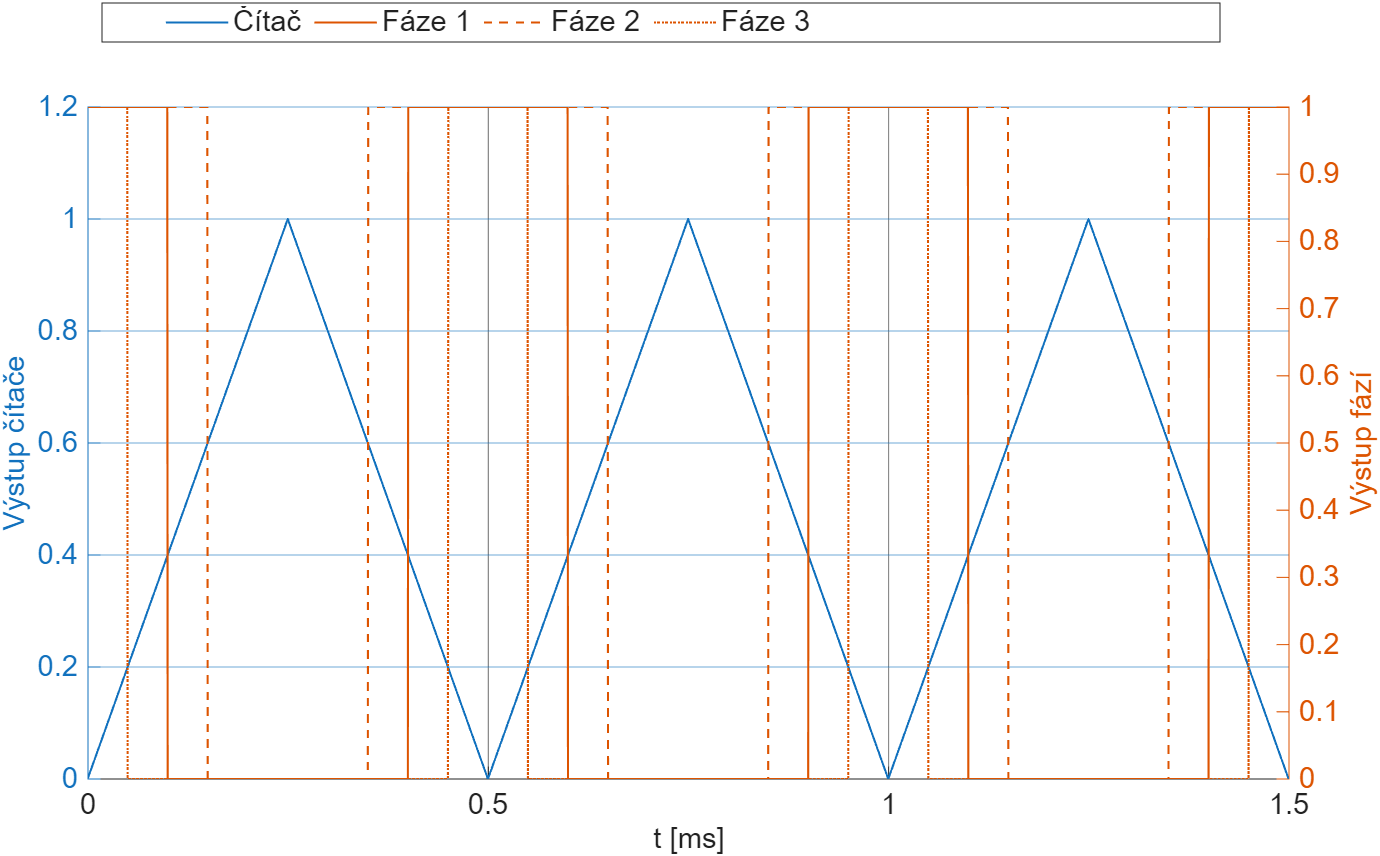
\includegraphics[width=\linewidth]{obrazky/Trazisotry.png}
    \caption{Výstup modulátoru pro horní tranzistory prvních 3 fází}
    \label{fig: sym modulace}
\end{figure}

Pro zjednodušenou simulaci je výstup jednotlivých fází převeden přímo na napětí na dané fázi vztahem \ref{eq: sw to u}, díky tomu si mohu dovolit simulaci provádět se simulační periodou odpovídající periodě modulace, to významně zrychluje simulaci a zjednodušuje mi práci s ostatními částmi kódu.
\begin{equation}
    \label{eq: sw to u}
    V_i=(V_{dc}\cdot sw_i)-\frac{V_{dc}}{2}
\end{equation}
Pro plnou simulaci a hardwarový výstup je výstupem bloku napětí, které by odpovídalo výstupu střídače v daný časový okamžik, tedy buď $-V_{dc}/2$ nebo $V_{dc}/2$.

\begin{figure}[h]
    \centering
    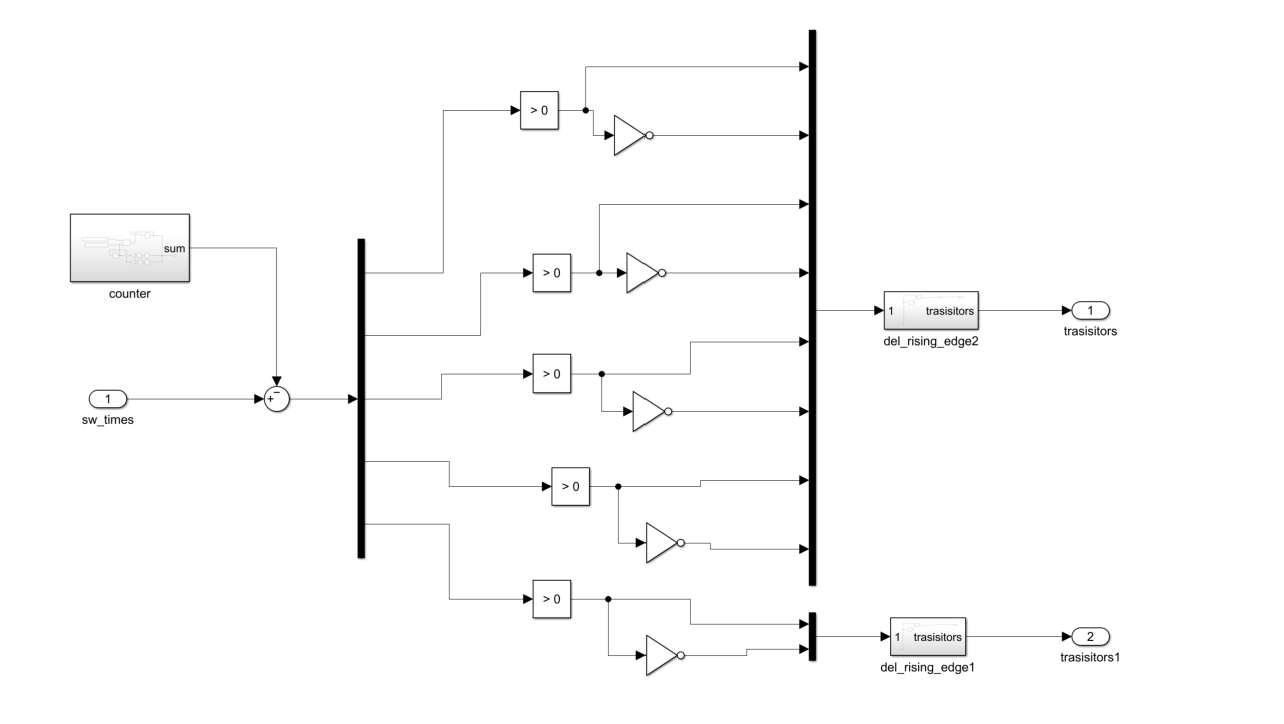
\includegraphics[width = \linewidth]{obrazky/hw_conecotr.png}
    \caption{Implementace vyvedení výstupu modulátoru v Simulinku}
\end{figure}

Pro testování potenciálního připojení tranzistorů na výstup jsem vytvořil blok \texttt{HW\_interface\_physicalPins}, který přivádí logické 0 nebo 1 na piny JA0--JA7 a JB1--JB2, na které by navazoval obvod s tranzistory určenými pro spínání jednotlivých fází.
Na obrázku \ref{fig: physical pins} je záznam z měření na osciloskopu, kde je vidět výstup z tohoto bloku. Pro zjednodušení jsou na obrázku viditelné průběhy pouze pro horní tranzistor první a druhé fáze. Lze vidět, že duty cycle odpovídající požadovaným hodnotám je pro první fázi 0{,}2 a pro druhou fázi 0{,}7.


\begin{figure}[!h]
    \centering
    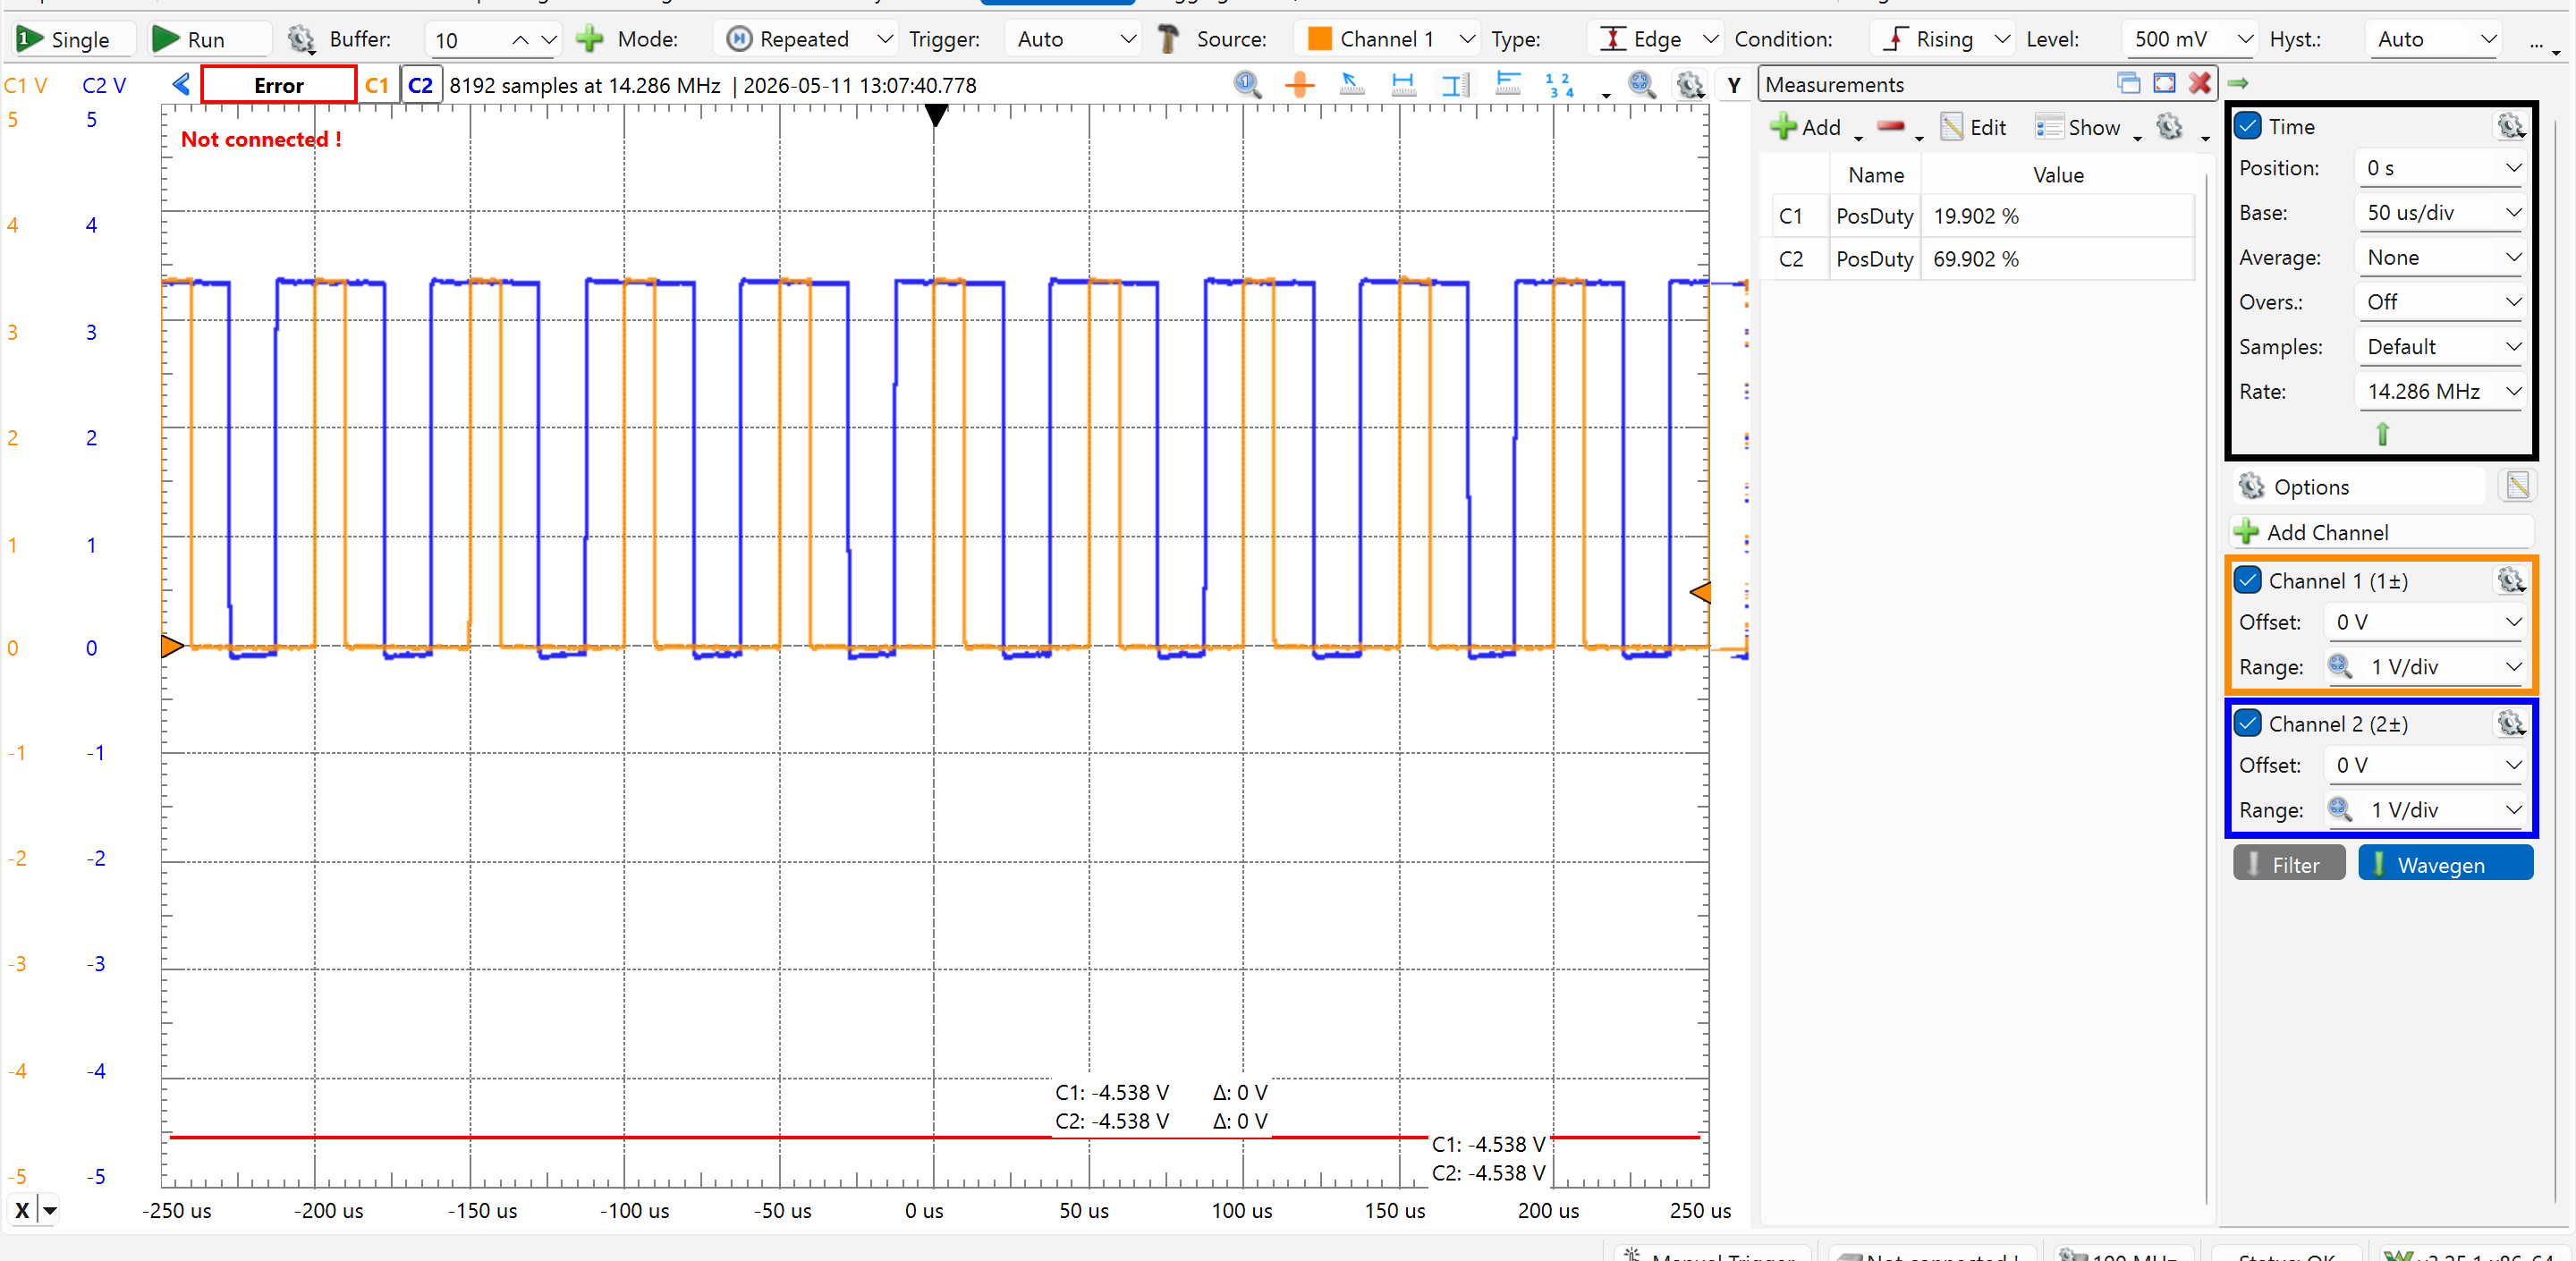
\includegraphics[width=\linewidth]{obrazky/osciloskop.png}
    \caption{Výstup měřený na fyzických pinech ZedBoardu. Oranžová -- pro první fázi $T_{sw\_1}=0{,}2$; Modrá -- pro druhou fázi $T_{sw\_2}=0{,}7$}
    \label{fig: physical pins}
\end{figure}    


\begin{table}[h]
\centering

\begin{tabular}{lrrrr}
\toprule
\textbf{Prostředek} & \textbf{Použito} & \textbf{Dostupné} & \textbf{[\%]} \\
\midrule
Slice LUT (celkem)       & 1\,557 & 53\,200  & 2{,}93 \\
\quad z toho: logika     & 1\,377 & 53\,200  & 2{,}59 \\
\quad z toho: dist. RAM  &   124  & 17\,400  & 0{,}71 \\
\quad z toho: shift reg. &    56  & 17\,400  & 0{,}32 \\
Slice Registers (FF)     & 2\,558 & 106\,400 & 2{,}40 \\
Block RAM tile           &     0  &    140   & 0{,}00 \\
DSP48E1 (násobičky)      &     0  &    220   & 0{,}00 \\
Slice                    &   735  & 13\,300  & 5{,}53 \\
\bottomrule
\end{tabular}
\caption{Využití HW prostředků FPGA -- vyvedení výstupu modulátoru (\texttt{HW\_Inteface\_Physical})}
\label{tab:hw_hdl_hwIntrface}
\end{table}



\subsection{Zpoždění při přepínání horní a dolní větve střídače}
Protože tranzistoru trvá nějakou dobu než se zavře, implementoval jsem zpoždění na náběžné hrany signálu pro tranzistory. Tím je zajištěno, že mezi vypnutím jednoho a sepnutím druhého tranzistoru stejné větve bude vždy mezera, která zajistí, že nedojde ke zkratu mezi napájecím napětím a zemí. Délka mezery je definována parametrem \texttt{DeadTime}. Zpoždění jde pozorovat ze záznamu z osciloskopu na obrázku \ref{fig: dead time}, kde je vidět, že mezi nástupem jednoho a druhého signálu je mezera, která zajišťuje, že nedojde ke zkratu.


\begin{figure}
    \centering
    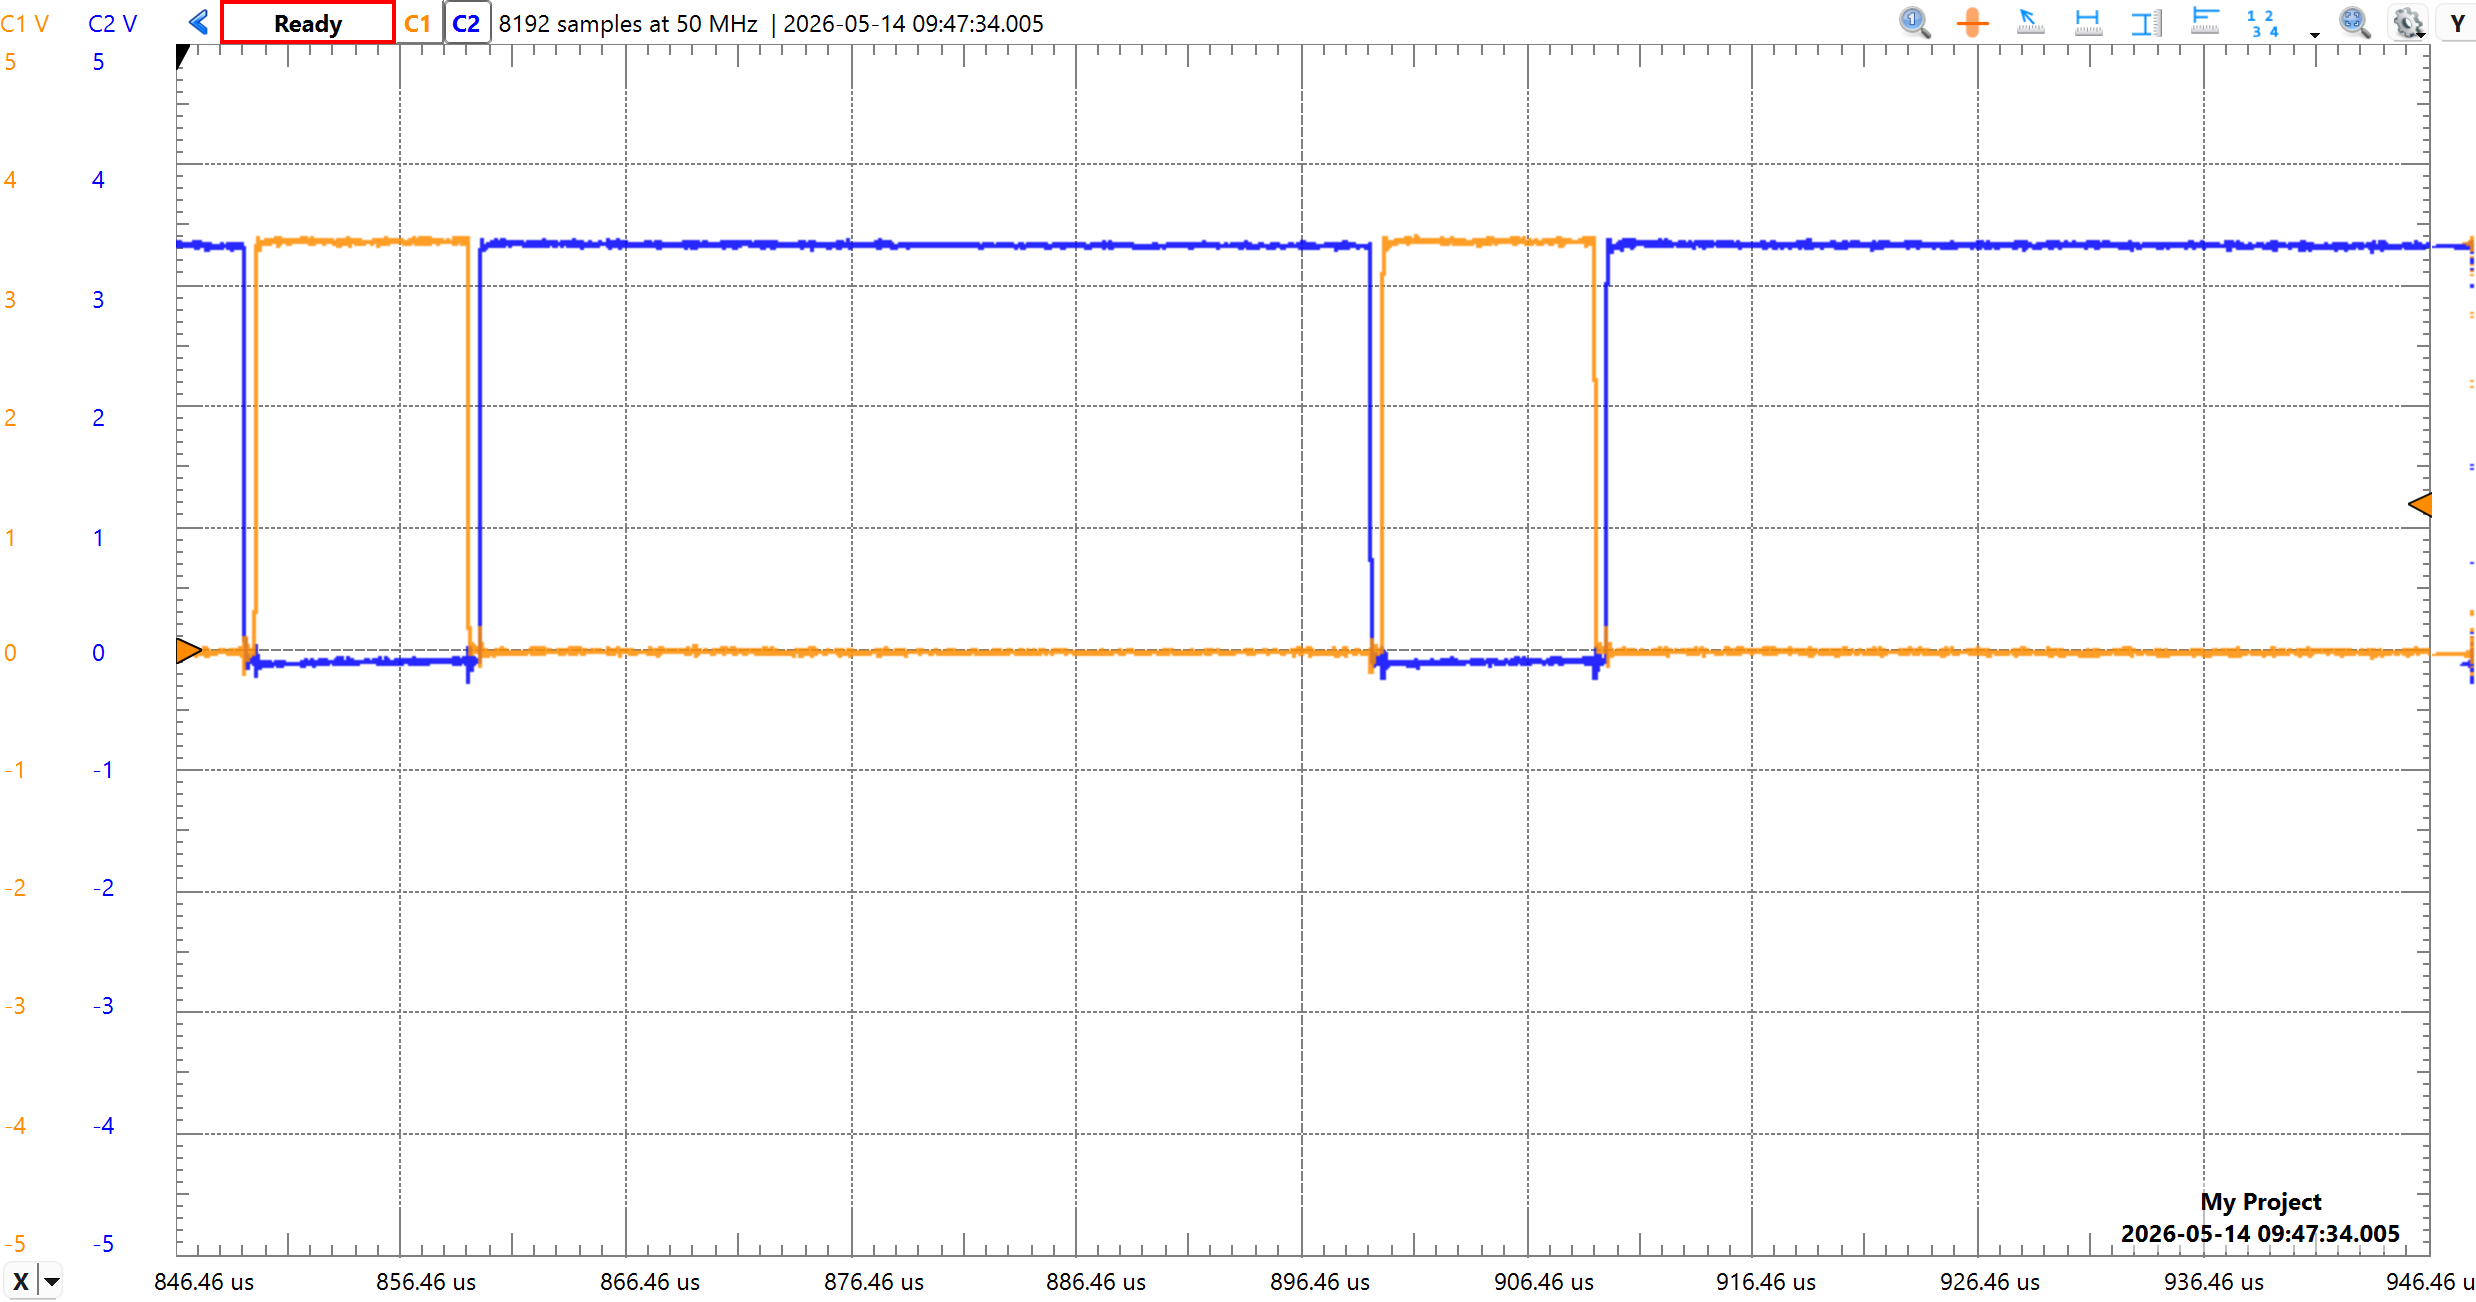
\includegraphics[width=\linewidth]{obrazky/osciloskop_deadtime.png}
    \caption{Zpoždění mezi nástupem signálu pro horní a dolní tranzistor stejné větve střídače}
    \label{fig: dead time}
\end{figure}

\section{Generování požadovaných proudů}
Jak je popsáno v kapitole \ref{kap:MTPA}, pro určení požadovaného proudu byla vygenerována lookup tabulka. Kvůli HDL implementaci je její použití rozděleno na 2 části: nejdříve je v první tabulce z požadovaného momentu určen nejbližší odpovídající index, ten slouží pro výběr odpovídajícího vektoru proudu z druhé lookup tabulky. Toto rozdělení je nutné proto, že indexování vícerozměrné tabulky v Matlabu lze realizovat pouze pomocí přirozených čísel. Pro jednodušší ladění a kontrolu funkčnosti zachovávám moment ve fyzikálních jednotkách; výpočet by mohl být zjednodušen normováním momentu. Implementace v Simulinku je na obrázku \ref{fig: T gen simulink}.

\begin{figure}[h]
    \centering
    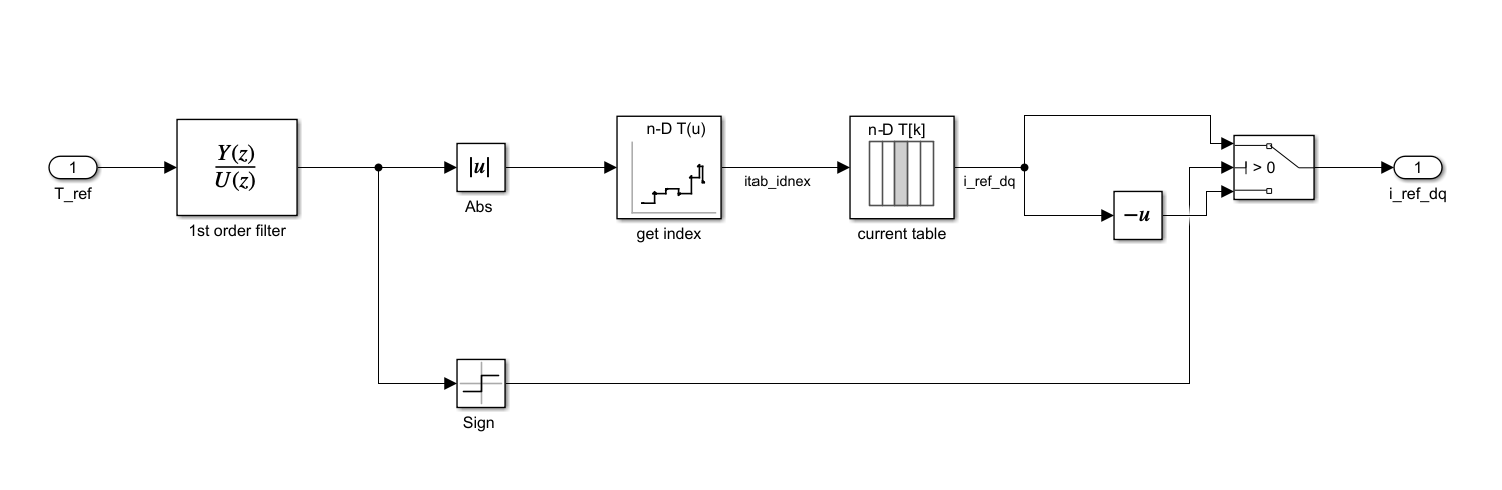
\includegraphics[width=\linewidth]{obrazky/T_gen_simulink.png}
    \caption{Implementace generování požadovaného proudu v simulinku}
    \label{fig: T gen simulink}
\end{figure}

Zároveň je v bloku ošetřen případný požadavek na záporný moment. Pokud je moment záporný, je na výstup vybrána větev s inverzními proudy.


Při rychlé změně momentu dochází ke skokové změně požadovaného proudu, což v některých případech způsobovalo kmitání momentu a v extrémních případech i nestabilitu celého řízení. Zároveň docházelo k překmitům proudů mimo povolený rozsah tranzistorů, průběhy jsou na obrázku \ref{fig:similnk moment proudy}. Proto jsem na vstup modulu přidal filtr žádané hodnoty s časovou konstantou 50\,ms.


Filtr je realizován jako dolní propust prvního řádu s přenosovou funkcí $F(p) = \frac{1}{1 + \tau p}$, kde $\tau = 50\,\text{ms}$. Hodnotu časové konstanty jsem zvolil experimentálně jako nejnižší hodnotu, při které byl výkyv proudů přijatelný. Filtr jsem pak použitím Eulerovy aproximace převedl na diskrétní ekvivalent, který je v bloku implementován. Vliv filtru na odezvu momentu je patrný z obrázku~\ref{fig:similnk moment}.


\begin{figure}[h]
    \centering
    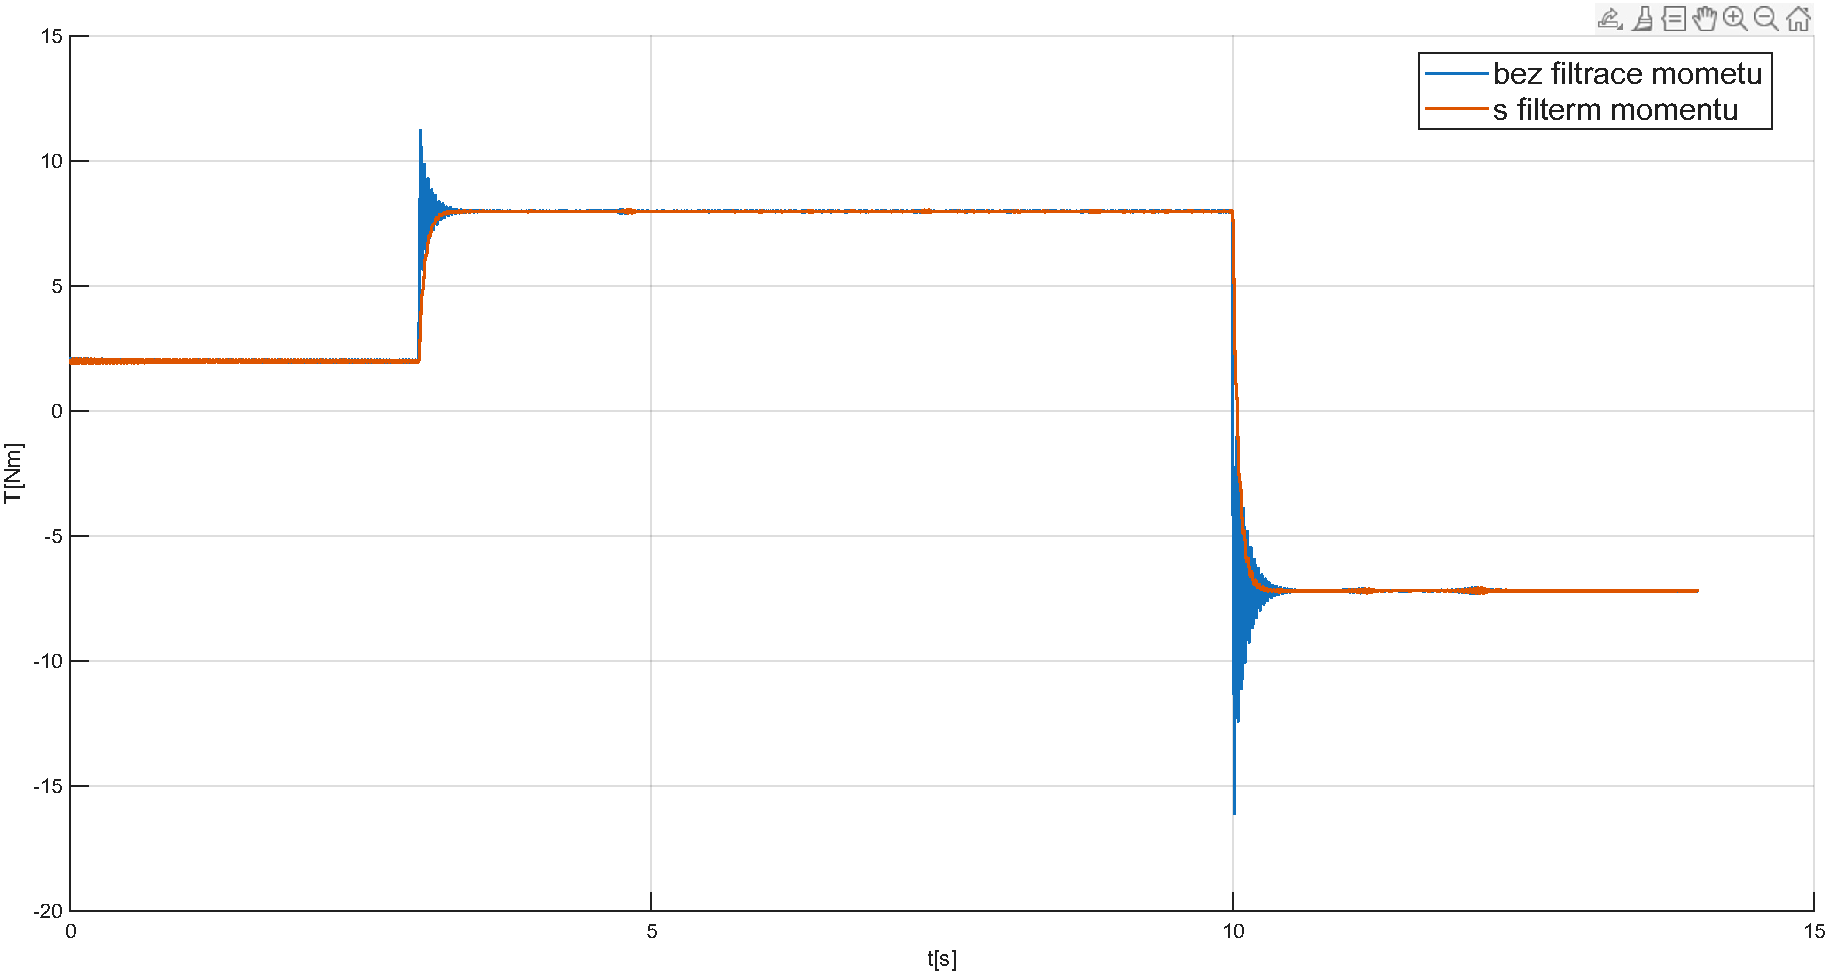
\includegraphics[width=0.9\linewidth]{obrazky/filtrT_moment.pdf}
    \caption{Porovnání odezvy systému na skokové změny momentu, s a bez filtru žádané hodnoty momentu}
    \label{fig:similnk moment}

    \vspace{1em}

    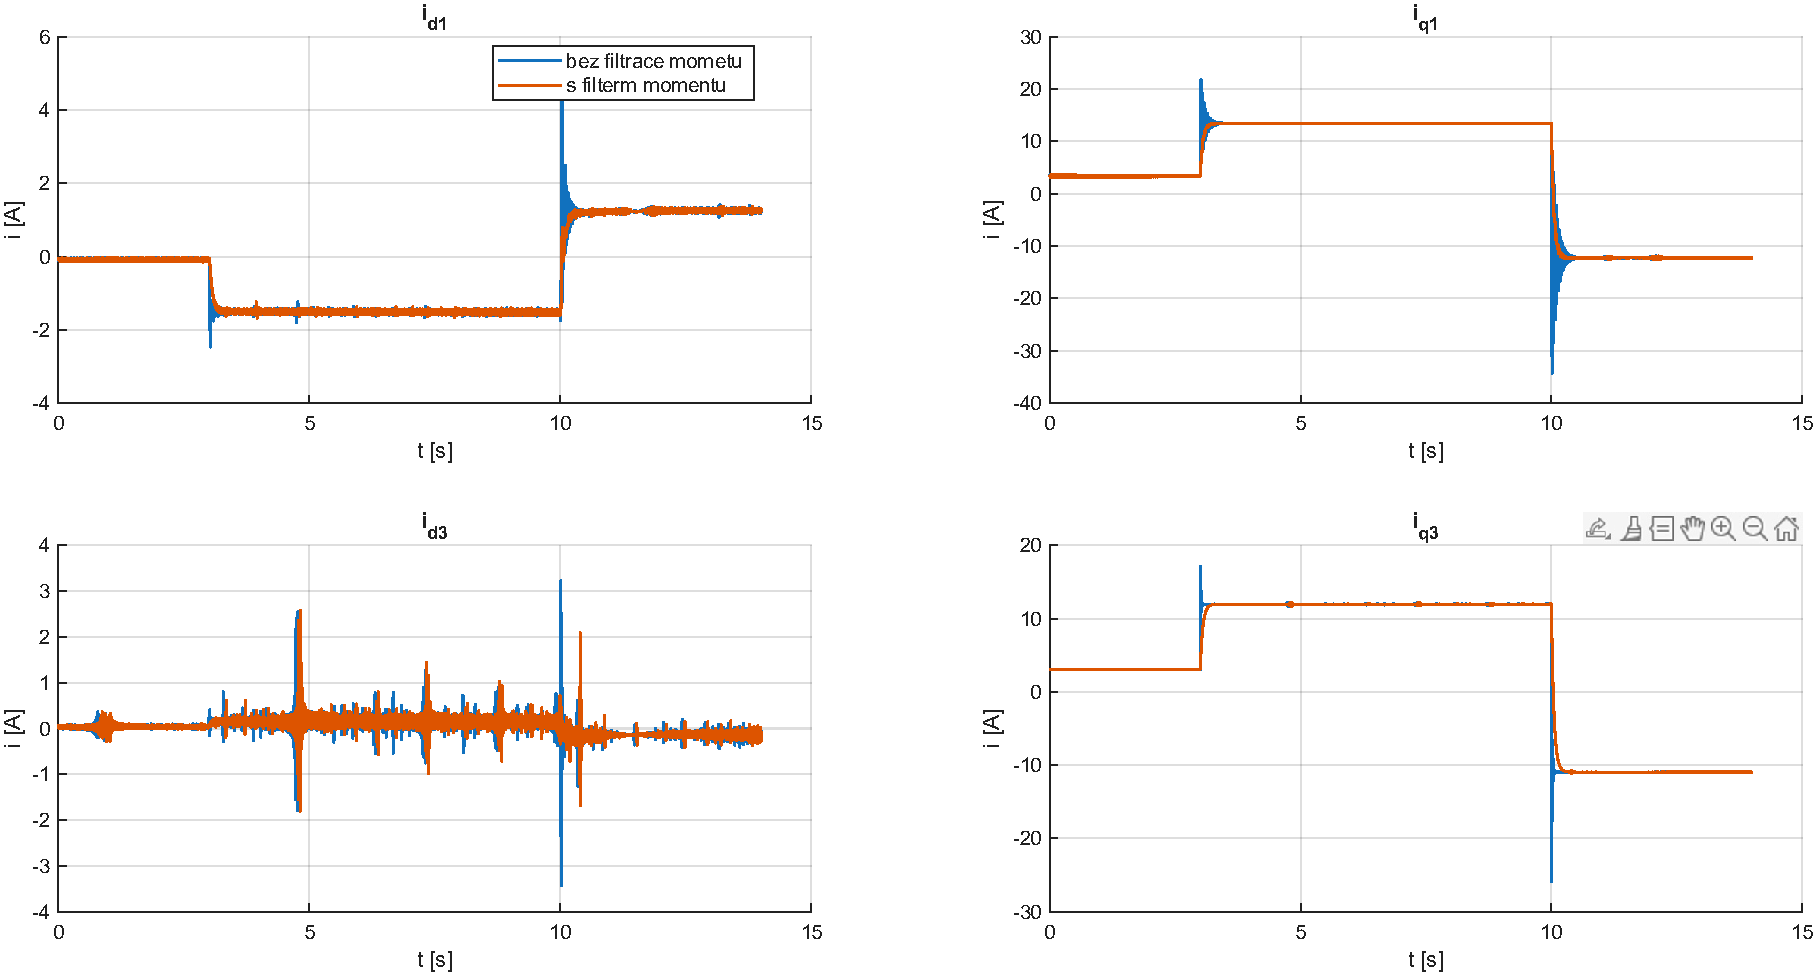
\includegraphics[width=0.9\linewidth]{obrazky/filtrT_proudy.pdf}
    \caption{Porovnání odezvy proudů na skokové změny momentu, s a bez filtru žádané hodnoty momentu}
    \label{fig:similnk moment proudy}
\end{figure}

Po provedení základních testů jsem se rozhodl MTPA použít přímo jako proudovou referenci bez implementace oslabování magnetického pole. Oslabování je relevantní pouze nad jmenovitými otáčkami, které jsem se v práci rozhodl nepřekračovat. Samotný výpočet kompenzačních proudů by byl výpočetně poměrně náročný. 

\begin{table}[h]
\centering
\begin{tabular}{lrrrr}
\toprule
\textbf{Prostředek} & \textbf{Použito} & \textbf{Dostupné} & \textbf{[\%]} \\
\midrule
Slice LUT (celkem)       & 6\,796 & 53\,200  & 12{,}77 \\
\quad z toho: logika     & 6\,619 & 53\,200  & 12{,}44 \\
\quad z toho: dist. RAM  &   116  & 17\,400  & 0{,}67 \\
\quad z toho: shift reg. &    61  & 17\,400  & 0{,}35 \\
Slice Registers (FF)     & 2\,313 & 106\,400 & 2{,}17 \\
RAMB36E1                 &     8  &    140   & 5{,}71 \\
RAMB18E1                 &     4  &    280   & 1{,}43 \\
Block RAM tile (celkem)  &    10  &    140   & 7{,}14 \\
DSP48E1 (násobičky)      &     1  &    220   & 0{,}45 \\
Slice                    & 2\,106 & 13\,300  & 15{,}83 \\
\bottomrule
\end{tabular}
\caption{Využití HW prostředků FPGA -- generování proudové reference (\texttt{tork\_gen})}
\label{tab:hw_hdl_Ttab}
\end{table}


\section{Regulátor otáček}
Regulaci otáček provádí PI regulátor, abych si zajistil plnou kontrolu nad datovými typy, implementoval jsem diskrétní verzi (PI) regulátor sám. Včetně antiwindupu. Aby regulátor zvládal rychle reagovat na změnu zatěžovacího momentu, který do systému z pohledu řízení vstupuje jako porucha, potřebuji výraznou I složku regulátoru, ta však způsobuje velký překmit při náběhu regulátoru, proto jsem i antiwindup naladil výrazně agresivněji.

Na obrázcích \ref{fig:speed reg} jsou vidět výsledky výsledné simulace celého systému. Požadované otáčky motoru se skokově mění po 5\,s a zároveň se s periodou 2,5\,s mění přídavná zátěž z 0 na 5\,Nm (\ref{fig:speed reg 2}). Na obrázcích je vidět, jak systém úspěšně zvládá jak skokové změny, tak poruchu. Na obr.~\ref{fig:speed reg 1} je zobrazen akční zásah (požadovaný moment) regulátoru otáček a jeho skutečná měřená hodnota.


\begin{figure}[!h]
    \centering
    \begin{subfigure}{\textwidth}
        \centering
        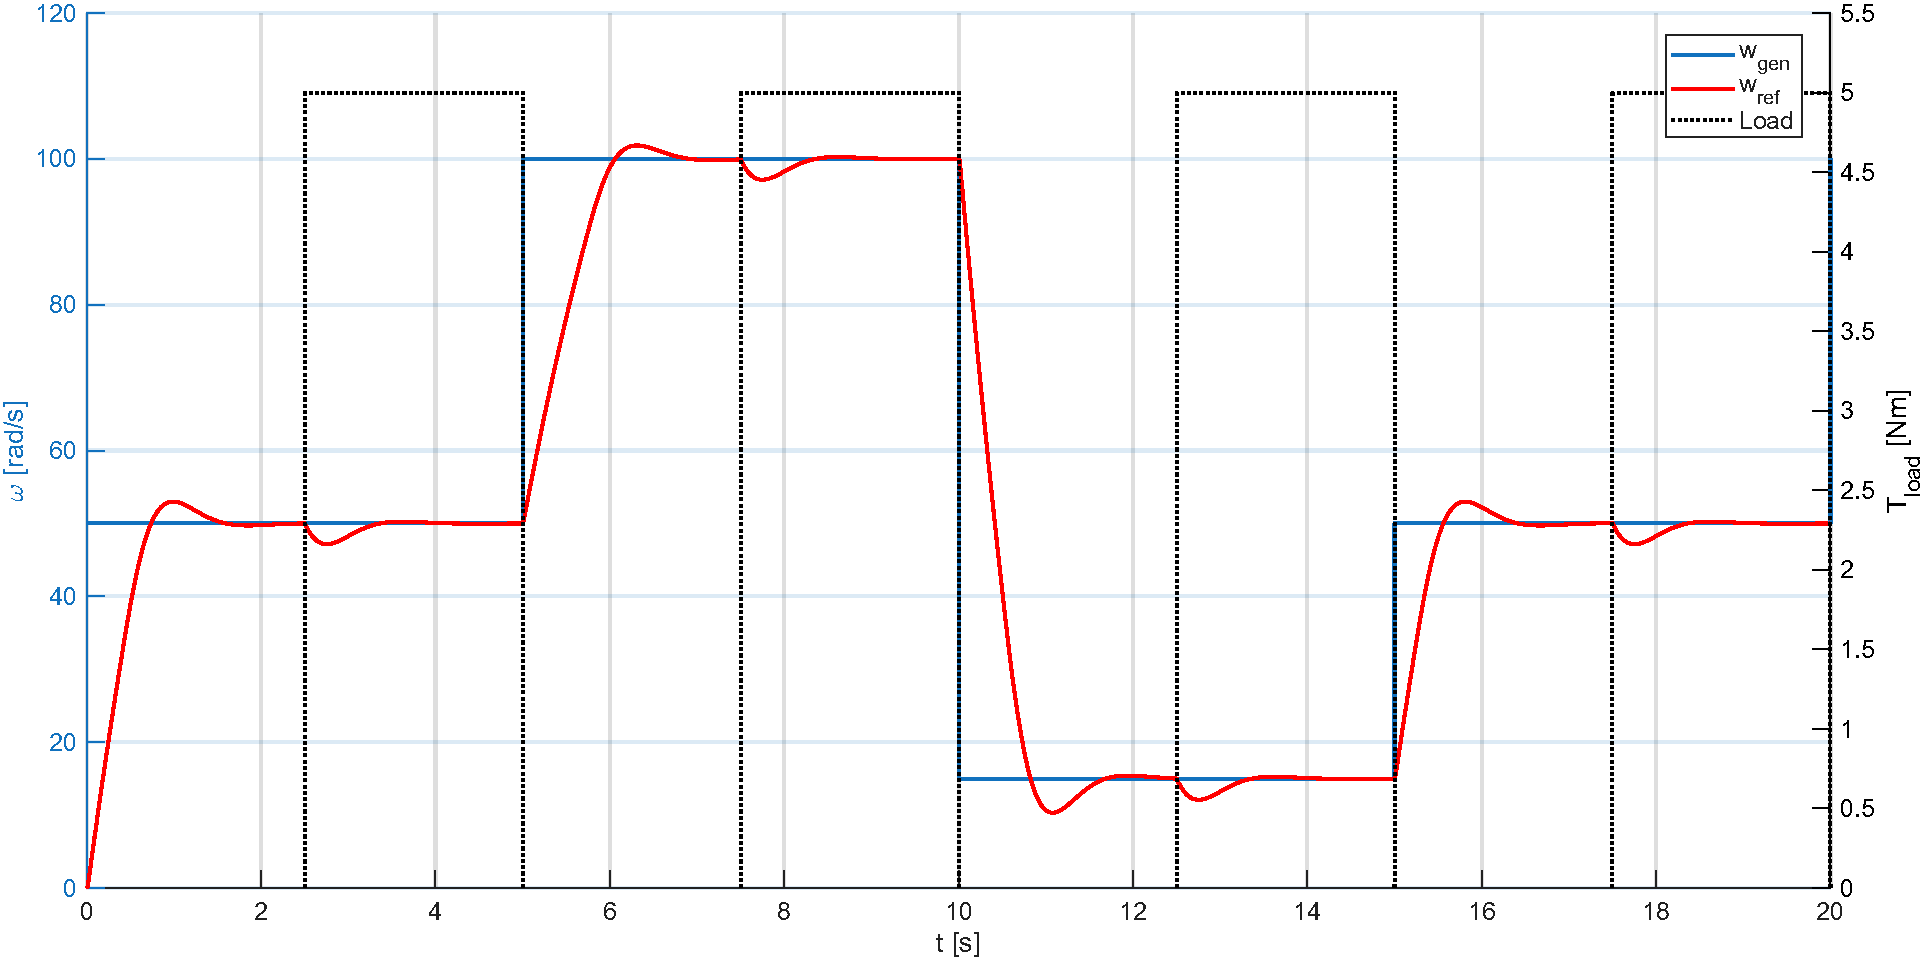
\includegraphics[width=\linewidth]{obrazky/speedReg2.pdf}
        \caption{Průběh rychlosti a zátěže}
        \label{fig:speed reg 2}
    \end{subfigure}

    \vspace{1em}

    \begin{subfigure}{\textwidth}
        \centering
        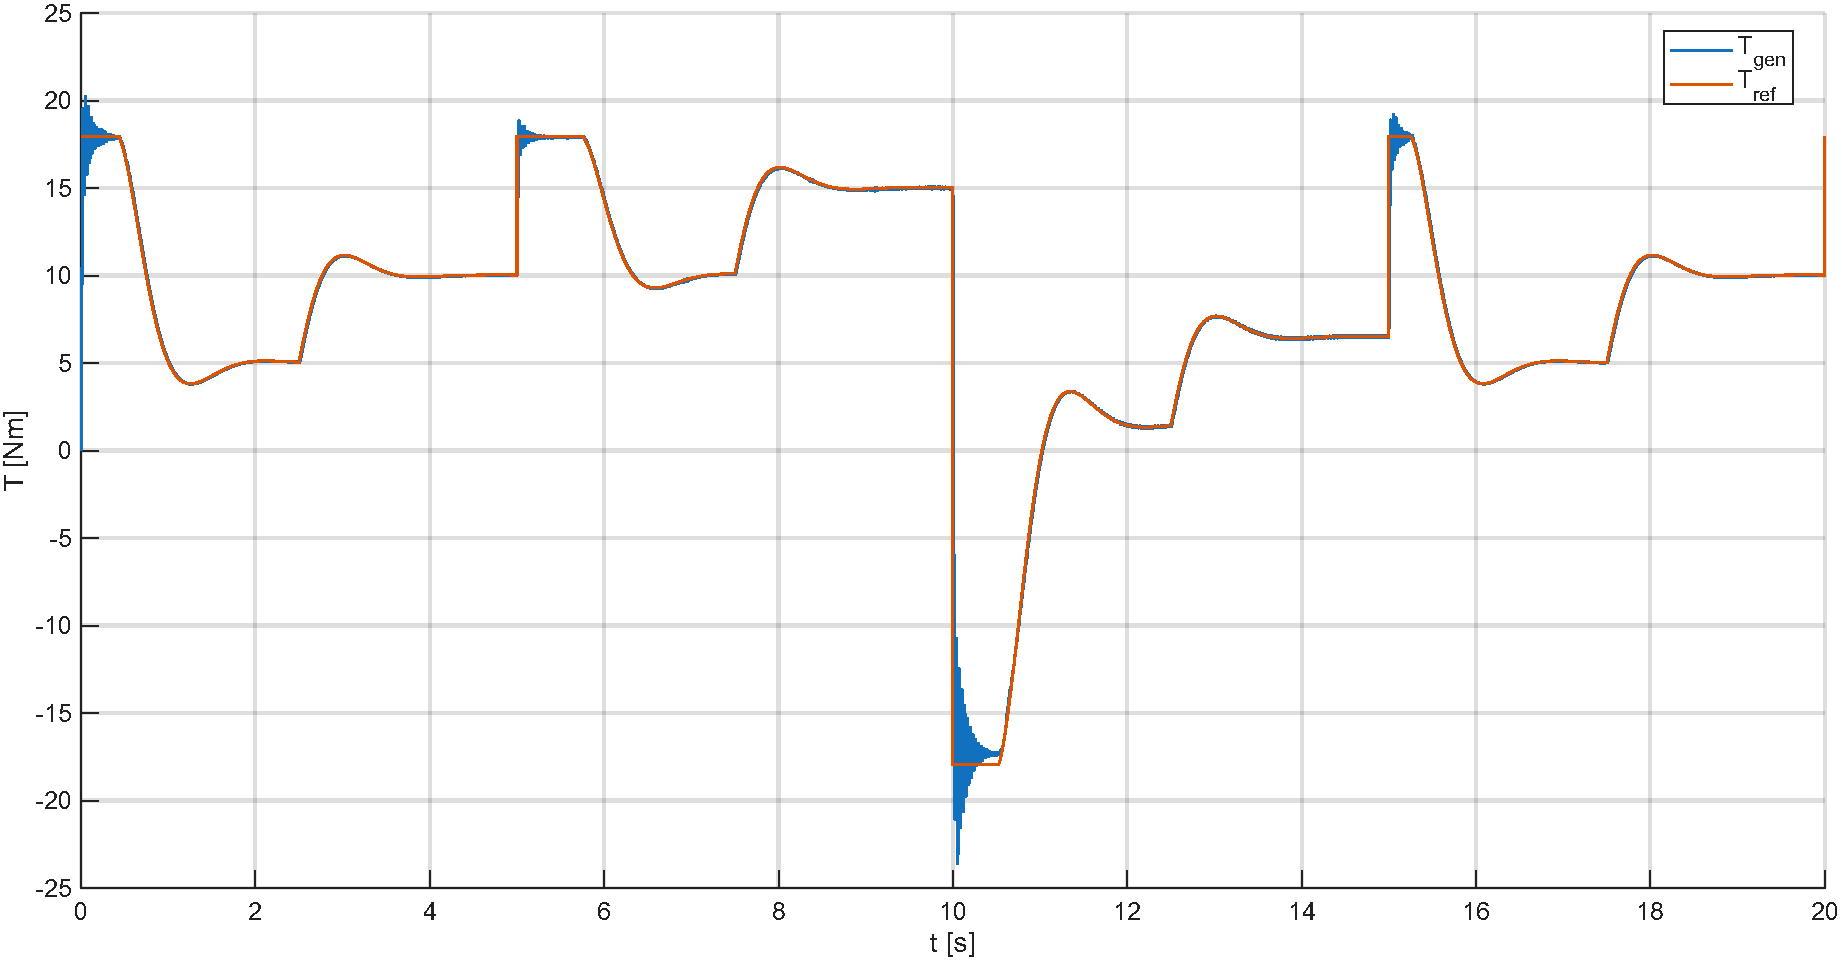
\includegraphics[width=\linewidth]{obrazky/speedReg1.pdf}
        \caption{Průběh momentu}
        \label{fig:speed reg 1}
    \end{subfigure}

    \caption{Výsledek simulace pro skokové změny otáček a zátěže}
    \label{fig:speed reg}
\end{figure}
 

\begin{table}[htbp]
\centering

\begin{tabular}{lrrrr}
\toprule
\textbf{Prostředek} & \textbf{Použito} & \textbf{Dostupné} & \textbf{[\%]} \\
\midrule
Slice LUT (celkem)       & 1\,578 & 53\,200  & 2{,}97 \\
\quad z toho: logika     & 1\,397 & 53\,200  & 2{,}63 \\
\quad z toho: dist. RAM  &   120  & 17\,400  & 0{,}69 \\
\quad z toho: shift reg. &    61  & 17\,400  & 0{,}35 \\
Slice Registers (FF)     & 2\,308 & 106\,400 & 2{,}17 \\
Block RAM tile           &     0  &    140   & 0{,}00 \\
DSP48E1 (násobičky)      &    10  &    220   & 4{,}55 \\
Slice                    &   820  & 13\,300  & 6{,}17 \\
\bottomrule
\end{tabular}
\caption{Využití HW prostředků FPGA -- regulátor rychlosti (\texttt{wreg})}
\label{tab:hw_hdlwreg}
\end{table}

\subsection{Proudový regulátor}
Pro každou z os je použit vlastní PI regulátor, který jsem implementoval sám. Má saturaci integrační složky a antiwindup. Na obrázku je verze s kompenzací křížové vazby. Součástí knihovny je i verze bez kompenzace.

\begin{figure}[h]
    \centering
    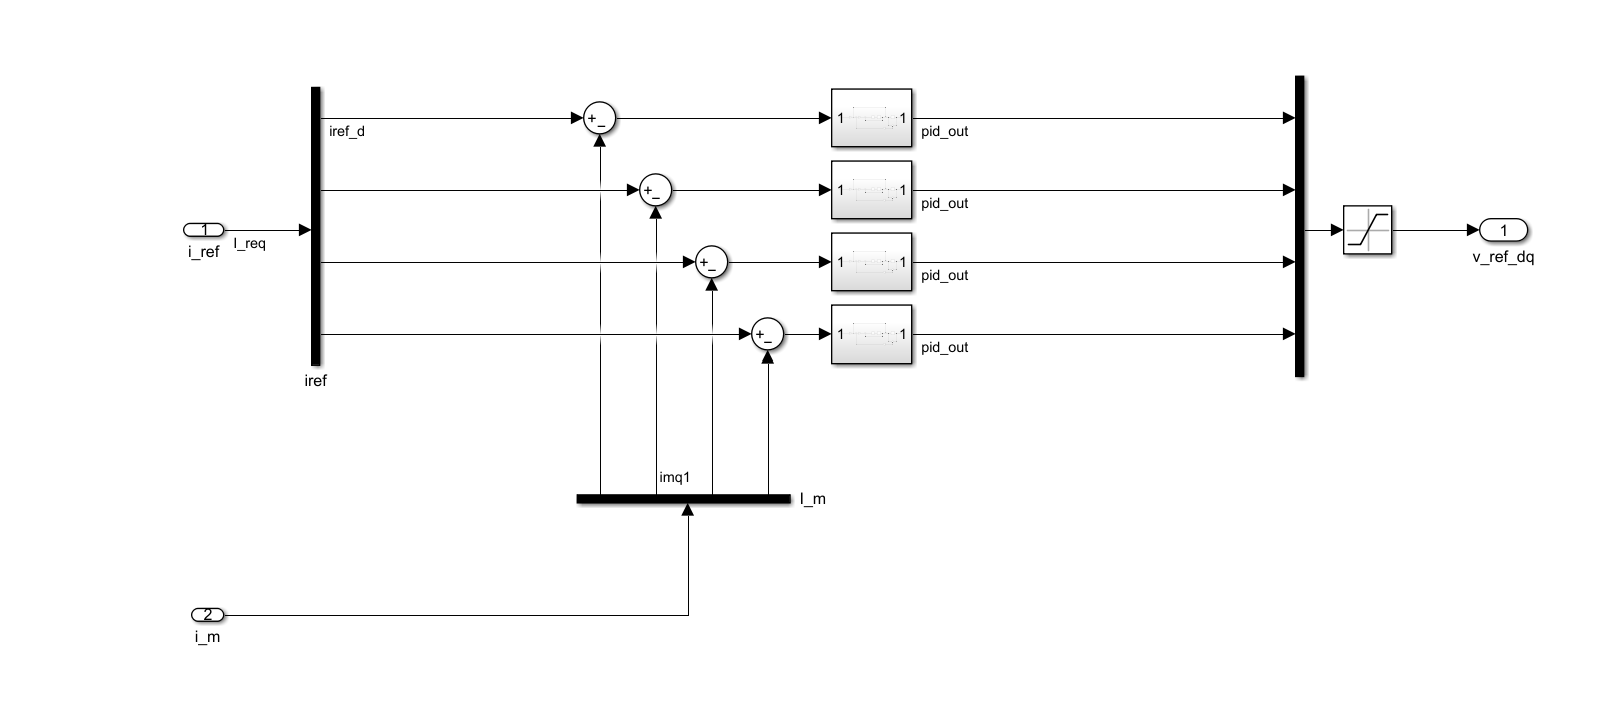
\includegraphics[width = \linewidth]{obrazky/ireg_sim.png}
    \caption{Implementace proudového regulátoru v Simulinku}
    \label{fig:simulink ire}
\end{figure} 

\begin{table}[htbp]
\centering

\begin{tabular}{lrrrr}
\toprule
\textbf{Prostředek} & \textbf{Použito} & \textbf{Dostupné} & \textbf{[\%]} \\
\midrule
Slice LUT (celkem)       & 3\,518 & 53\,200  & 6{,}61 \\
\quad z toho: logika     & 3\,333 & 53\,200  & 6{,}27 \\
\quad z toho: dist. RAM  &   124  & 17\,400  & 0{,}71 \\
\quad z toho: shift reg. &    61  & 17\,400  & 0{,}35 \\
Slice Registers (FF)     & 2\,809 & 106\,400 & 2{,}64 \\
Block RAM tile           &     0  &    140   & 0{,}00 \\
DSP48E1 (násobičky)      &   102  &    220   & 46{,}36 \\
Slice                    & 1\,253 & 13\,300  & 9{,}42 \\
\bottomrule
\end{tabular}
\caption{Využití HW prostředků FPGA -- regulátor proudu (\texttt{Ireg})}
\label{tab:hw_hdl_prj}
\end{table}


\section{Implementace na ZedBoard}

V této kapitole je představen vývojový kit SoC, na kterém je řízení počítáno. Je rozebrána náročnost jednotlivých funkcí, vybrány datové reprezentace jednotlivých signálů a popsány dosažené výsledky.

\begin{figure}[!h]
    \centering
    \resizebox{0.8 \textwidth}{!}{
    

\begin{tikzpicture}[
    % Styly pro jednotlivé prvky
    block/.style={draw, rectangle, minimum width=3.5cm, minimum height=1.2cm, align=center, fill=white, font=\sffamily},
    container/.style={draw, thick, rectangle, inner sep=15pt, fill=gray!10, rounded corners},
    arrow/.style={-{Stealth[scale=1.2]}, thick},
    connection/.style={font=\sffamily\small}
]

% --- ZEDBOARD (Levá strana) ---
% Vnitřní bloky
\node[block] (reg) {Regulátor};
\node[block, below=0.8cm of reg] (mod) {Modulátor};

% Kontejner ZedBoard
\begin{scope}[on background layer]
    \node[container, fit=(reg)(mod), label={[font=\sffamily\bfseries]above:ZedBoard}] (zed) {};
\end{scope}

% --- SIMULINK NA PC (Pravá strana) ---
% Vnitřní bloky
\node[block, right=6cm of reg] (motor) {Model motoru};
\node[block, below=0.8cm of motor] (disp) {Zobrazení\\výsledků};

% Kontejner Simulink
\begin{scope}[on background layer]
    \node[container, fit=(motor)(disp), label={[font=\sffamily\bfseries]above:Simulink na PC}] (simbox) {};
\end{scope}

% --- PROPOJENÍ (Ethernet) ---
% Šipka směrem do PC (Akční zásahy)
\draw[arrow] ([yshift=1cm]zed.east) -- ([yshift=1cm]simbox.west) 
    node[midway, above, connection] {Akční zásahy};

% Šipka směrem do ZedBoardu (Měřené veličiny)
\draw[arrow] ($(simbox.west)+(0,-1cm)$) -- ($(zed.east)+(0,-1cm)$)
    node[midway, below, connection] {Měřené veličiny v abcde};

% Štítek sběrnice/sítě
\node at ($(zed.east)!0.5!(simbox.west)$) [fill=white, draw=black!50, rounded corners, inner sep=4pt, font=\sffamily\bfseries\small] {Ethernet};

% --- VNITŘNÍ VAZBY (Volitelné, dokreslují tok signálu uvnitř zařízení) ---
\draw[arrow, dashed, draw=black!60] (reg) -- (mod);
\draw[arrow, dashed, draw=black!60] (motor) -- (disp);

\end{tikzpicture}
}
    \caption{Schéma simulace s řídícím hardwarem zahrnutým v simulační smyčce}
    \label{fig:HIL}
\end{figure}

Protože fyzický pohon nemám k dispozici, provádím v práci pouze simulaci s HIL (Hardware in the Loop) se ZedBoard deskou ve smyčce. Na vývojovou desku jsou ze Simulinku zasílány údaje o měření z modelu a ZedBoard vrací akční zásahy zpět.
Komunikace probíhá přes Ethernet, kterým je počítač propojen přímo s vývojovou deskou. Pohon je simulován na počítači v prostředí Simulink.


\subsection{ZedBoard}

ZedBoard je vývojová deska navržená společností Digilent ve spolupráci se společností Xilinx. Deska je určena pro vývoj a prototypování aplikací na obvodu Zynq-7000 SoC. Na desce jsou k dispozici standardní rozhraní jako HDMI, USB, Ethernet, SD karta, tlačítka a přepínače pro rychlé ověření funkce vyvíjeného systému. Pro účely propojení s výkonovou elektronikou pohonu jsou pak využívány konektory PMOD a FMC, které umožňují připojení externích periferií.

ZedBoard je vývojový kit postavený na obvodu Xilinx Zynq-7020, který patří do rodiny Zynq-7000 SoC (System on Chip). Obvod kombinuje dvě části: procesorový subsystém (PS) tvořený dvojicí jader ARM Cortex-A9 taktovaných až na 667\,MHz a programovatelnou logiku (PL) odpovídající čipu Artix-7. Pro tuto práci je stěžejní část PL, na níž je implementováno řízení motoru ve formě IP cores generovaných z prostředí Simulink HDL Coder.\cite{zedBoard1} \cite{zedBoard2}

\subsubsection{Paměti}

Programovatelná logika čipu XC7Z020 disponuje dvěma druhy interní paměti. Prvním jsou bloky Block RAM (BRAM), druhým je distribuovaná paměť realizovaná pomocí LUT buněk.

Čip obsahuje 140 bloků Block RAM, přičemž každý blok má kapacitu 36\,kb. Celková kapacita Block RAM je tedy $140 \times 36\,\text{kb} = 4{,}9\,\text{Mb}$. Každý blok lze nakonfigurovat buď jako jeden blok RAMB36 (hloubka až 32\,K $\times$ 1\,b nebo 1\,K $\times$ 36\,b), nebo jako dva nezávislé bloky RAMB18 (hloubka až 16\,K $\times$ 1\,b nebo 512 $\times$ 36\,b). Paměti BRAM jsou využity zejména pro lookup tabulky hodnot $\sin$ a $\cos$, které jsou popsány v kapitole věnované transformacím.\cite{zedBoard1} \cite{zedBoard2}


\subsubsection{Násobiče}

Z hlediska implementace aritmetiky je klíčová dostupnost hardwarových násobiček. Čip XC7Z020 obsahuje 220 bloků DSP48E1, které jsou primárním prostředkem pro realizaci násobení v PL. Každý blok DSP48E1 obsahuje:
\begin{itemize}
    \item přednásobičkový sčítač se šířkou 27\,bitů (pre-adder),
    \item násobiče se vstupy o šířce 27~bitů (výsledek násobení se tedy vejde do 45\,bitů),
    \item 48\,bitový akumulátor s volitelnou kaskádou.
\end{itemize}

Bloky DSP48E1 lze kaskádně řetězit, čímž je možné realizovat operace jako skalární součin nebo filtr bez nutnosti použití dalších logických buněk. Mimo bloky DSP48E1 je možné násobení realizovat také v logice LUT, avšak za cenu vyššího využití programovatelné logiky a nižší maximální frekvence. Nástroj HDL Coder při syntéze automaticky mapuje operace násobení na DSP48E1, pokud to šířka operandů umožňuje.\cite{zedBoard1} \cite{zedBoard2}

Celkový počet logických buněk PL čipu XC7Z020 je 53\,200 LUT a 106\,400 klopných obvodů (flip-flop). Přehled klíčových zdrojů PL je shrnut v tabulce~\ref{tab:zedboard_zdroje}.\cite{zedBoard1} \cite{zedBoard2}

\begin{table}[h]
    \centering
    \begin{tabular}{|l|r|}
    \hline 
    Zdroj & Počet / Kapacita \\ \hline
    LUT (6-vstupové) & 53\,200 \\
    Klopné obvody (FF) & 106\,400 \\
    Bloky DSP48E1 & 220 \\
    Bloky Block RAM (36\,kb) & 140 \\
    Celková kapacita Block RAM & 4{,}9\,Mb \\
    Externí DDR3 SDRAM & 512\,MB \\ \hline
    \end{tabular}
    \caption{Přehled klíčových zdrojů PL čipu XC7Z020 na desce ZedBoard}
    \label{tab:zedboard_zdroje}
\end{table}

\subsection{Datové typy}
V práci jsem zachoval fyzikální rozměry veličin, pro generování HDL kódu bylo potřeba převést datové typy jednotlivých signálů na datové typy s pevnou desetinnou čárkou. U každého signálu musí být definována délka proměnné v bitech, informace zda nabývá veličina i záporných hodnot a počet bitů reprezentujících, kolik z celkové délky proměnné je vyhrazeno na cast za desetinnou čárkou (fraction).

Soupis využitých datových typů pro jednotlivé signály je shrnut v tabulce \ref{tab:datove_typy}. Po testování jsem volil rozsah kolem 20 bitů, při kterých systém plynule sledoval požadovanou hodnotu. Cílem bylo pokud možno nepřesáhnout délku násobiče na ZedBoard 27 bitů. U většiny datových typů by šlo dále snižovat jejich bitový rozsah, se stávajícím nastavením se celý výpočet vejde na ZedBoard, ponechal jsem je tedy na těchto hodnotách, abych docílil lepší odezvy.

Úhel natočení jsem pro jednodušší reprezentaci převedl z radiánů na zlomky otáčky, úhel tedy nabývá hodnot od 0 do 1.

\begin{table}[h]
    \centering
    \begin{tabular}{|l|c|c|c|l|}
        \hline
        \textbf{signál} & \textbf{délka [bit]} & \textbf{znaménkový} & \textbf{bitové dělení } & \textbf{MATLAB definice} \\ \hline
        proud ($i$)     & 20                  & ano (1)             & 13                                & \texttt{fixdt(1,20,13)} \\ \hline
        úhel ($ang$)    & 20                  & ne (0)              & 17                                & \texttt{fixdt(0,20,17)} \\ \hline
        napětí ($u$)    & 27                  & ano (1)             & 18                                & \texttt{fixdt(1,27,18)} \\ \hline
        spínací časy ($swt$) & 20                  & ano (1)             & 18                                & \texttt{fixdt(1,20,18)} \\ \hline
        moment ($T$)    & 15                  & ano (1)             & 8                                 & \texttt{fixdt(1,15,8)}  \\ \hline
        otáčky ($w$)    & 16                  & ano (1)             & 5                                 & \texttt{fixdt(1,16,5)}  \\ \hline
    \end{tabular}
    \caption{Datové typy signálů použité pro generování HDL}
    \label{tab:datove_typy}
\end{table}

\subsection{Využití jednotlivých zdrojů}
V tabulce \ref{tab:hw_utilization_summary} je souhrn využití zdrojů jednotlivých bloků, včetně potřebných zdrojů na IP core pokrývající kompletní regulaci motoru. Nejvíce je využito bloků násobiček (DSP48) -- 88\,\% možných. Nejvíce jich spotřebuje blok proudového regulátoru, zejména kvůli velkému násobení signálů s dlouhou bitovou délkou. Regulátor bez kompenzace křížové vazby potřebuje přibližně o polovinu méně DSP bloků.

Pokud by bylo nutné výpočetní náročnost dále snižovat, bylo by nutné měnit přesnost jednotlivých datových typů.


\begin{table}[htbp]
\centering
\small
\setlength{\tabcolsep}{4pt}
\begin{threeparttable}
\begin{tabular}{p{4.5cm}rrrrrr}
    \toprule
    \textbf{Blok}
    & \textbf{LUT}
    & \textbf{FF}
    & \textbf{LUT RAM}
    & \textbf{BRAM}
    & \textbf{DSP48}
    & \textbf{Slice} \\
    \midrule
    \multicolumn{7}{l}{\textit{Dostupné prostředky}} \\
    \quad Celkem na čipu
    & 53\,200 & 106\,400 & 17\,400 & 280
    & 220 & 13\,300 \\
    \midrule
    \multicolumn{7}{l}{\textit{Jednotlivé bloky}} \\
    Inverzní transformace do $\alpha \beta_{1\,3}$ 
    & 2\,106 & 2\,668 & 124 & 0 & 48 & 1\,083 \\
    \quad využití [\%]
    & 3{,}96 & 2{,}51 & 0{,}71 & 0{,}00 & 21{,}82 & 8{,}14 \\
    \addlinespace
    Regulátor momentu
    & 1\,578 & 2\,308 & 120 & 0 & 10 & 820 \\
    \quad využití [\%]
    & 2{,}97 & 2{,}17 & 0{,}69 & 0{,}00 & 4{,}55 & 6{,}17 \\
    \addlinespace
    Regulátor proudu
    & 3\,518 & 2\,809 & 124 & 0 & 102 & 1\,253 \\
    \quad využití [\%]
    & 6{,}61 & 2{,}64 & 0{,}71 & 0{,}00 & 46{,}36 & 9{,}42 \\
    \addlinespace
    Proudový regulátor bez kompenzace křížové vazby
    & 2\,934 & 2\,809 & 124 & 0 & 54 & 1\,138 \\
    \quad využití [\%]
    & 5{,}52 & 2{,}64 & 0{,}71 & 0{,}00 & 24{,}55 & 8{,}56 \\
    \addlinespace
    Transformace do $dq_{1\,3}$
    & 8\,917 & 2\,918 & 126 & 0 & 48 & 3\,342 \\
    \quad využití [\%]
    & 16{,}76 & 2{,}74 & 0{,}72 & 0{,}00 & 21{,}82 & 25{,}13 \\
    \addlinespace
    HW rozhraní 
    & 1\,557 & 2\,558 & 124 & 0 & 0 & 735 \\
    \quad využití [\%]
    & 2{,}93 & 2{,}40 & 0{,}71 & 0{,}00 & 0{,}00 & 5{,}53 \\
    \addlinespace
    Generování proudové reference
    & 6\,796 & 2\,313 & 116 & 20
    & 1 & 2\,106 \\
    \quad využití [\%]
    & 12{,}77 & 2{,}17 & 0{,}67 & 7{,}14 & 0{,}45 & 15{,}83 \\
    \addlinespace
    \textbf{Celý systém \texttt{hdl\_celek}}
    & \textbf{13\,933} & \textbf{4\,197} & \textbf{124} & \textbf{20} & \textbf{195} & \textbf{4\,361} \\
    \quad využití [\%]
    & \textbf{26{,}19} & \textbf{3{,}94} & \textbf{0{,}71} & \textbf{7{,}14} & \textbf{88{,}64} & \textbf{32{,}79} \\

    \bottomrule
\end{tabular}
\begin{tablenotes}
    \small
    \item LUT – Look-Up Table (logická buňka); FF – Flip-Flop (registr);
    LUT RAM – LUT použité jako distribuovaná RAM;
    BRAM – Block RAM (36\,kb tile); DSP48 – DSP48E1 (násobičko-akumulátor).
\end{tablenotes}
\end{threeparttable}
\caption{Přehled využití hardwarových prostředků jednotlivými bloky a celkem}
\label{tab:hw_utilization_summary}
\end{table}



%\begin{table}[htbp]
%\centering
%\caption{Využití HW prostředků FPGA -- celý systém (\texttt{hdl\_celek}).
%         Zařízení: xc7z020clg484-1, stav: Fully Placed.}
%\label{tab:hw_hdl_celek}
%\begin{tabular}{lrrrr}
%\toprule
%\textbf{Prostředek} & \textbf{Použito} & \textbf{Dostupné} & \textbf{[\%]} \\
%\midrule
%Slice LUT (celkem)       & 13\,933 & 53\,200  & 26{,}19 \\
%\quad z toho: logika     & 13\,733 & 53\,200  & 25{,}81 \\
%\quad z toho: dist. RAM  &    124  & 17\,400  & 0{,}71 \\
%\quad z toho: shift reg. &     76  & 17\,400  & 0{,}44 \\
%Slice Registers (FF)     &  4\,197 & 106\,400 & 3{,}94 \\
%RAMB36E1                 &      8  &    140   & 5{,}71 \\
%RAMB18E1                 &      4  &    280   & 1{,}43 \\
%Block RAM tile (celkem)  &     10  &    140   & 7{,}14 \\
%DSP48E1 (násobičky)      &    195  &    220   & 88{,}64 \\
%Slice                    &  4\,361 & 13\,300  & 32{,}79 \\
%\bottomrule
%\end{tabular}
%\end{table}
